% Generated fragments require trusted human review before compilation.
% This binder never requests shell escape or runs external tools.
\documentclass[11pt]{article}
% Trusted shared apparatus. Requires LuaLaTeX; never use shell escape.
\usepackage{fontspec}
\defaultfontfeatures{Ligatures=TeX}
\IfFontExistsTF{Noto Serif}{\setmainfont{Noto Serif}}{%
  \IfFontExistsTF{DejaVu Serif}{\setmainfont{DejaVu Serif}}{%
    \IfFontExistsTF{Times New Roman}{\setmainfont{Times New Roman}}{%
      \PackageError{gelfand-binder}{No configured Cyrillic serif font installed}{Install Noto Serif or DejaVu Serif, or select an installed Cyrillic font.}%
    }%
  }%
}
\IfFontExistsTF{Noto Sans}{\setsansfont{Noto Sans}}{%
  \IfFontExistsTF{DejaVu Sans}{\setsansfont{DejaVu Sans}}{\setsansfont{Arial}}%
}
\IfFontExistsTF{Noto Sans Mono}{\setmonofont{Noto Sans Mono}}{%
  \IfFontExistsTF{DejaVu Sans Mono}{\setmonofont{DejaVu Sans Mono}}{\setmonofont{Courier New}}%
}
\usepackage[a4paper,margin=22mm]{geometry}
\usepackage{amsmath,amssymb,amsthm,mathtools}
\usepackage{xcolor}
\usepackage{tikz}
\usepackage{tikz-cd}
\usetikzlibrary{arrows.meta,positioning,calc}
\usepackage{hyperref}
\hypersetup{unicode=true,colorlinks=true,linkcolor=blue,pdftitle={Gelfand transcription binder}}
\newtheorem{theorem}{Theorem}
\newtheorem{lemma}{Lemma}
\newtheorem{proposition}{Proposition}
\newtheorem{corollary}{Corollary}
\theoremstyle{definition}
\newtheorem{definition}{Definition}
\newtheorem{example}{Example}
\theoremstyle{remark}
\newtheorem{remark}{Remark}
\setlength{\parindent}{0pt}
\setlength{\parskip}{0.55em}
\setlength{\emergencystretch}{3em}
\newcommand{\SourcePage}[2]{%
  \clearpage\phantomsection\label{#1:source-page}%
  \addcontentsline{toc}{subsection}{#1}%
  {\small\sffamily\color{blue!60!black}Source scan frame: #1; visible page/leaf label: #2}\par\medskip%
}
\newcommand{\Unclear}[3]{%
  \begingroup\color{orange!70!black}%
  [Unresolved reading #1/#2: #3]\endgroup%
}
\newcommand{\Incomplete}[3]{%
  \par\begingroup\color{red!65!black}\textbf{Incomplete #1/#2:} #3\endgroup\par%
}
\newcommand{\SourceFigure}[3]{%
  \par\begingroup\color{blue!60!black}\textbf{\hyperref[#1:source-page]{Source figure #1/#2}:} #3%
  \par\textit{Consult the authoritative scan at this locator.}\endgroup\par%
}



% Reader layout only. Original diplomatic text is retained verbatim.
\setlength{\parskip}{0.35em}
\setlength{\emergencystretch}{4em}
\renewcommand{\SourcePage}[2]{%
  \par\addvspace{1em}\noindent\leavevmode\phantomsection\label{#1:source-page}%
  \addcontentsline{toc}{subsection}{#1}%
  {\footnotesize\sffamily\color{blue!55!black}#1%
    \def\givenlabel{#2}\def\nolabel{unlabelled}%
    \ifx\givenlabel\nolabel\else\quad[номер в источнике: #2]\fi
  }\par\nobreak\smallskip%
}
\renewcommand{\Unclear}[3]{%
  \begingroup\color{orange!65!black}%
  \ifmmode\text{[неясно: #3]}\else[неясно: #3]\fi\endgroup%
}
\renewcommand{\Incomplete}[3]{%
  \par\begingroup\color{red!60!black}\textbf{Неразобранный фрагмент:} #3%
  \endgroup\par%
}
\renewcommand{\SourceFigure}[3]{%
  \par\begingroup\color{blue!55!black}\textbf{Рисунок:} #3%
  \par{\small\textit{Исходный рисунок: \hyperref[#1:source-page]{#1}, #2.}}%
  \endgroup\par%
}
\hypersetup{pdftitle={Семинар И. М. Гельфанда. Дипломатическая транскрипция},pdfauthor={},pdfsubject={Русское рабочее издание с отмеченными сомнительными чтениями}}

\usepackage[normalem]{ulem}
\usepackage{newunicodechar}
\usepackage{adjustbox}
\newfontfamily\SourceSymbolFont{Segoe UI Symbol}
\newfontfamily\SourceCJKFont{MS Gothic}
\let\DiplomaticMathUnderline\underline
\renewcommand{\underline}[1]{\ifmmode\DiplomaticMathUnderline{#1}\else\uline{#1}\fi}
\newunicodechar{→}{\ifmmode\text{{\SourceSymbolFont\char"2192}}\else{\SourceSymbolFont\char"2192}\fi}
\newunicodechar{⇒}{\ifmmode\text{{\SourceSymbolFont\char"21D2}}\else{\SourceSymbolFont\char"21D2}\fi}
\newunicodechar{∀}{\ifmmode\text{{\SourceSymbolFont\char"2200}}\else{\SourceSymbolFont\char"2200}\fi}
\newunicodechar{∂}{\ifmmode\text{{\SourceSymbolFont\char"2202}}\else{\SourceSymbolFont\char"2202}\fi}
\newunicodechar{∈}{\ifmmode\text{{\SourceSymbolFont\char"2208}}\else{\SourceSymbolFont\char"2208}\fi}
\newunicodechar{∌}{\ifmmode\text{{\SourceSymbolFont\char"220C}}\else{\SourceSymbolFont\char"220C}\fi}
\newunicodechar{√}{\ifmmode\text{{\SourceSymbolFont\char"221A}}\else{\SourceSymbolFont\char"221A}\fi}
\newunicodechar{∞}{\ifmmode\text{{\SourceSymbolFont\char"221E}}\else{\SourceSymbolFont\char"221E}\fi}
\newunicodechar{∧}{\ifmmode\text{{\SourceSymbolFont\char"2227}}\else{\SourceSymbolFont\char"2227}\fi}
\newunicodechar{∩}{\ifmmode\text{{\SourceSymbolFont\char"2229}}\else{\SourceSymbolFont\char"2229}\fi}
\newunicodechar{∪}{\ifmmode\text{{\SourceSymbolFont\char"222A}}\else{\SourceSymbolFont\char"222A}\fi}
\newunicodechar{∫}{\ifmmode\text{{\SourceSymbolFont\char"222B}}\else{\SourceSymbolFont\char"222B}\fi}
\newunicodechar{∴}{\ifmmode\text{{\SourceSymbolFont\char"2234}}\else{\SourceSymbolFont\char"2234}\fi}
\newunicodechar{∼}{\ifmmode\text{{\SourceSymbolFont\char"223C}}\else{\SourceSymbolFont\char"223C}\fi}
\newunicodechar{≈}{\ifmmode\text{{\SourceSymbolFont\char"2248}}\else{\SourceSymbolFont\char"2248}\fi}
\newunicodechar{≠}{\ifmmode\text{{\SourceSymbolFont\char"2260}}\else{\SourceSymbolFont\char"2260}\fi}
\newunicodechar{≤}{\ifmmode\text{{\SourceSymbolFont\char"2264}}\else{\SourceSymbolFont\char"2264}\fi}
\newunicodechar{≥}{\ifmmode\text{{\SourceSymbolFont\char"2265}}\else{\SourceSymbolFont\char"2265}\fi}
\newunicodechar{⊕}{\ifmmode\text{{\SourceSymbolFont\char"2295}}\else{\SourceSymbolFont\char"2295}\fi}
\newunicodechar{⊗}{\ifmmode\text{{\SourceSymbolFont\char"2297}}\else{\SourceSymbolFont\char"2297}\fi}
\newunicodechar{①}{\ifmmode\text{{\SourceSymbolFont\char"2460}}\else{\SourceSymbolFont\char"2460}\fi}
\newunicodechar{②}{\ifmmode\text{{\SourceSymbolFont\char"2461}}\else{\SourceSymbolFont\char"2461}\fi}
\newunicodechar{③}{\ifmmode\text{{\SourceSymbolFont\char"2462}}\else{\SourceSymbolFont\char"2462}\fi}
\newunicodechar{④}{\ifmmode\text{{\SourceSymbolFont\char"2463}}\else{\SourceSymbolFont\char"2463}\fi}
\newunicodechar{Ⓗ}{\ifmmode\text{{\SourceSymbolFont\char"24BD}}\else{\SourceSymbolFont\char"24BD}\fi}
\newunicodechar{〃}{\ifmmode\text{{\SourceCJKFont\char"3003}}\else{\SourceCJKFont\char"3003}\fi}


% Reader revision 3. Annotation wording and candidates remain unchanged.
\setmainfont{NotoSerif-Regular.ttf}[Path=C:/Windows/Fonts/,ItalicFont=NotoSerif-Italic.ttf,BoldFont=NotoSerif-Bold.ttf,BoldItalicFont=NotoSerif-BoldItalic.ttf]
\usetikzlibrary{shapes.geometric,decorations.pathreplacing,decorations.markings,patterns,fit}
\newsavebox{\ReaderAnnotationBox}
\newcommand{\ReaderAnnotation}[1]{%
  \sbox{\ReaderAnnotationBox}{[неясно: #1]}%
  \ifdim\wd\ReaderAnnotationBox>.70\linewidth
    \parbox[t]{.70\linewidth}{\raggedright[неясно: #1]}%
  \else\usebox{\ReaderAnnotationBox}\fi%
}
\ExplSyntaxOn
\cs_new_protected:Npn \reader_unclear_candidate:n #1
 {
  \tl_set:Nx \l_tmpa_tl { \tl_to_str:n {#1} }
  % Text explicitly guarded inside a mathematical candidate remains math-safe.
  \regex_replace_all:nnN { \\(?:text|textrm|textnormal|textbf|operatorname)\s*\{[^{}]*\} } { } \l_tmpa_tl
  \regex_match:nVTF { [\x{0400}-\x{052F}] | \$ } \l_tmpa_tl
   { \ifmmode \text{\ReaderAnnotation{#1}} \else \ReaderAnnotation{#1} \fi }
   {
    \ifmmode
      [\text{неясно:~}#1]
    \else
      \regex_match:nVTF { [_^] | \\ } \l_tmpa_tl
       { \ensuremath{[\text{неясно:~}#1]} }
       { \ReaderAnnotation{#1} }
    \fi
   }
 }
\RenewDocumentCommand \Unclear { m m m }
 { \begingroup\color{orange!65!black}\reader_unclear_candidate:n{#3}\endgroup }
\ExplSyntaxOff
\newsavebox{\ReaderIncompleteBox}
\newcommand{\ReaderIncompleteNote}[1]{%
 \sbox{\ReaderIncompleteBox}{\textbf{Неразобранный фрагмент:} #1}%
 \ifdim\wd\ReaderIncompleteBox>.70\linewidth
  \parbox[t]{.70\linewidth}{\raggedright\textbf{Неразобранный фрагмент:} #1}%
 \else\usebox{\ReaderIncompleteBox}\fi%
}
\renewcommand{\Incomplete}[3]{%
 \ifmmode\text{\color{red!60!black}\ReaderIncompleteNote{#3}}%
 \else\leavevmode\begingroup\color{red!60!black}\ReaderIncompleteNote{#3}\endgroup\fi%
}
% Ragged right avoids stretching long untranslated abbreviations into margins.
\AtBeginDocument{\raggedright}
\newunicodechar{А}{\ifmmode\text{\char"410\relax}\else\char"410\relax\fi}
\newunicodechar{Б}{\ifmmode\text{\char"411\relax}\else\char"411\relax\fi}
\newunicodechar{В}{\ifmmode\text{\char"412\relax}\else\char"412\relax\fi}
\newunicodechar{Г}{\ifmmode\text{\char"413\relax}\else\char"413\relax\fi}
\newunicodechar{Д}{\ifmmode\text{\char"414\relax}\else\char"414\relax\fi}
\newunicodechar{Е}{\ifmmode\text{\char"415\relax}\else\char"415\relax\fi}
\newunicodechar{Ж}{\ifmmode\text{\char"416\relax}\else\char"416\relax\fi}
\newunicodechar{З}{\ifmmode\text{\char"417\relax}\else\char"417\relax\fi}
\newunicodechar{И}{\ifmmode\text{\char"418\relax}\else\char"418\relax\fi}
\newunicodechar{Й}{\ifmmode\text{\char"419\relax}\else\char"419\relax\fi}
\newunicodechar{К}{\ifmmode\text{\char"41A\relax}\else\char"41A\relax\fi}
\newunicodechar{Л}{\ifmmode\text{\char"41B\relax}\else\char"41B\relax\fi}
\newunicodechar{М}{\ifmmode\text{\char"41C\relax}\else\char"41C\relax\fi}
\newunicodechar{Н}{\ifmmode\text{\char"41D\relax}\else\char"41D\relax\fi}
\newunicodechar{О}{\ifmmode\text{\char"41E\relax}\else\char"41E\relax\fi}
\newunicodechar{П}{\ifmmode\text{\char"41F\relax}\else\char"41F\relax\fi}
\newunicodechar{Р}{\ifmmode\text{\char"420\relax}\else\char"420\relax\fi}
\newunicodechar{С}{\ifmmode\text{\char"421\relax}\else\char"421\relax\fi}
\newunicodechar{Т}{\ifmmode\text{\char"422\relax}\else\char"422\relax\fi}
\newunicodechar{У}{\ifmmode\text{\char"423\relax}\else\char"423\relax\fi}
\newunicodechar{Ф}{\ifmmode\text{\char"424\relax}\else\char"424\relax\fi}
\newunicodechar{Х}{\ifmmode\text{\char"425\relax}\else\char"425\relax\fi}
\newunicodechar{Ц}{\ifmmode\text{\char"426\relax}\else\char"426\relax\fi}
\newunicodechar{Ч}{\ifmmode\text{\char"427\relax}\else\char"427\relax\fi}
\newunicodechar{Ш}{\ifmmode\text{\char"428\relax}\else\char"428\relax\fi}
\newunicodechar{Щ}{\ifmmode\text{\char"429\relax}\else\char"429\relax\fi}
\newunicodechar{Ъ}{\ifmmode\text{\char"42A\relax}\else\char"42A\relax\fi}
\newunicodechar{Ы}{\ifmmode\text{\char"42B\relax}\else\char"42B\relax\fi}
\newunicodechar{Ь}{\ifmmode\text{\char"42C\relax}\else\char"42C\relax\fi}
\newunicodechar{Э}{\ifmmode\text{\char"42D\relax}\else\char"42D\relax\fi}
\newunicodechar{Ю}{\ifmmode\text{\char"42E\relax}\else\char"42E\relax\fi}
\newunicodechar{Я}{\ifmmode\text{\char"42F\relax}\else\char"42F\relax\fi}
\newunicodechar{а}{\ifmmode\text{\char"430\relax}\else\char"430\relax\fi}
\newunicodechar{б}{\ifmmode\text{\char"431\relax}\else\char"431\relax\fi}
\newunicodechar{в}{\ifmmode\text{\char"432\relax}\else\char"432\relax\fi}
\newunicodechar{г}{\ifmmode\text{\char"433\relax}\else\char"433\relax\fi}
\newunicodechar{д}{\ifmmode\text{\char"434\relax}\else\char"434\relax\fi}
\newunicodechar{е}{\ifmmode\text{\char"435\relax}\else\char"435\relax\fi}
\newunicodechar{ж}{\ifmmode\text{\char"436\relax}\else\char"436\relax\fi}
\newunicodechar{з}{\ifmmode\text{\char"437\relax}\else\char"437\relax\fi}
\newunicodechar{и}{\ifmmode\text{\char"438\relax}\else\char"438\relax\fi}
\newunicodechar{й}{\ifmmode\text{\char"439\relax}\else\char"439\relax\fi}
\newunicodechar{к}{\ifmmode\text{\char"43A\relax}\else\char"43A\relax\fi}
\newunicodechar{л}{\ifmmode\text{\char"43B\relax}\else\char"43B\relax\fi}
\newunicodechar{м}{\ifmmode\text{\char"43C\relax}\else\char"43C\relax\fi}
\newunicodechar{н}{\ifmmode\text{\char"43D\relax}\else\char"43D\relax\fi}
\newunicodechar{о}{\ifmmode\text{\char"43E\relax}\else\char"43E\relax\fi}
\newunicodechar{п}{\ifmmode\text{\char"43F\relax}\else\char"43F\relax\fi}
\newunicodechar{р}{\ifmmode\text{\char"440\relax}\else\char"440\relax\fi}
\newunicodechar{с}{\ifmmode\text{\char"441\relax}\else\char"441\relax\fi}
\newunicodechar{т}{\ifmmode\text{\char"442\relax}\else\char"442\relax\fi}
\newunicodechar{у}{\ifmmode\text{\char"443\relax}\else\char"443\relax\fi}
\newunicodechar{ф}{\ifmmode\text{\char"444\relax}\else\char"444\relax\fi}
\newunicodechar{х}{\ifmmode\text{\char"445\relax}\else\char"445\relax\fi}
\newunicodechar{ц}{\ifmmode\text{\char"446\relax}\else\char"446\relax\fi}
\newunicodechar{ч}{\ifmmode\text{\char"447\relax}\else\char"447\relax\fi}
\newunicodechar{ш}{\ifmmode\text{\char"448\relax}\else\char"448\relax\fi}
\newunicodechar{щ}{\ifmmode\text{\char"449\relax}\else\char"449\relax\fi}
\newunicodechar{ъ}{\ifmmode\text{\char"44A\relax}\else\char"44A\relax\fi}
\newunicodechar{ы}{\ifmmode\text{\char"44B\relax}\else\char"44B\relax\fi}
\newunicodechar{ь}{\ifmmode\text{\char"44C\relax}\else\char"44C\relax\fi}
\newunicodechar{э}{\ifmmode\text{\char"44D\relax}\else\char"44D\relax\fi}
\newunicodechar{ю}{\ifmmode\text{\char"44E\relax}\else\char"44E\relax\fi}
\newunicodechar{я}{\ifmmode\text{\char"44F\relax}\else\char"44F\relax\fi}
\newunicodechar{Ё}{\ifmmode\text{\char"401\relax}\else\char"401\relax\fi}
\newunicodechar{ё}{\ifmmode\text{\char"451\relax}\else\char"451\relax\fi}

\newunicodechar{æ}{\ifmmode\text{\char"E6\relax}\else\char"E6\relax\fi}
\newunicodechar{−}{\ifmmode\mathbin{\text{\SourceSymbolFont\char"2212\relax}}\else{\SourceSymbolFont\char"2212\relax}\fi}


% Reader-only pairing support; accepted raw bodies remain unchanged.
\RequirePackage{graphicx}
\RequirePackage{adjustbox}
\newcommand{\ReaderOriginalPanel}[2]{%
  \begin{minipage}[t]{.48\linewidth}\vspace{0pt}\centering
    \includegraphics[width=\linewidth,keepaspectratio]{#1}\par\smallskip
    {\scriptsize Оригинал рукописного рисунка: #2}\par
  \end{minipage}%
}
\newcommand{\ReaderDiagramPair}[3]{%
  \par\noindent\begingroup
  \ReaderOriginalPanel{#1}{#2}\hfill
  \begin{minipage}[t]{.48\linewidth}\vspace{0pt}\centering
    {\scriptsize Типографское воссоздание}\par\smallskip
    \begin{adjustbox}{max width=\linewidth}#3\end{adjustbox}\par
  \end{minipage}%
  \endgroup\par\smallskip
}
\newcommand{\ReaderDescriptionPair}[3]{%
  \par\noindent\begingroup
  \ReaderOriginalPanel{#1}{#2}\hfill
  \begin{minipage}[t]{.48\linewidth}\vspace{0pt}\raggedright
    {\scriptsize Типографское описание}\par\smallskip
    #3\par
  \end{minipage}%
  \endgroup\par\smallskip
}


\newunicodechar{ℂ}{\ifmmode\text{{\SourceSymbolFont\char"2102\relax}}\else{\SourceSymbolFont\char"2102\relax}\fi}
\newunicodechar{∇}{\ifmmode\text{{\SourceSymbolFont\char"2207\relax}}\else{\SourceSymbolFont\char"2207\relax}\fi}
\newunicodechar{∐}{\ifmmode\text{{\SourceSymbolFont\char"2210\relax}}\else{\SourceSymbolFont\char"2210\relax}\fi}
\newunicodechar{∑}{\ifmmode\text{{\SourceSymbolFont\char"2211\relax}}\else{\SourceSymbolFont\char"2211\relax}\fi}
\newunicodechar{∘}{\ifmmode\text{{\SourceSymbolFont\char"2218\relax}}\else{\SourceSymbolFont\char"2218\relax}\fi}
\newunicodechar{≅}{\ifmmode\text{{\SourceSymbolFont\char"2245\relax}}\else{\SourceSymbolFont\char"2245\relax}\fi}
\newunicodechar{⊂}{\ifmmode\text{{\SourceSymbolFont\char"2282\relax}}\else{\SourceSymbolFont\char"2282\relax}\fi}
\newunicodechar{⟨}{\ifmmode\text{{\SourceSymbolFont\char"27E8\relax}}\else{\SourceSymbolFont\char"27E8\relax}\fi}
\newunicodechar{⟩}{\ifmmode\text{{\SourceSymbolFont\char"27E9\relax}}\else{\SourceSymbolFont\char"27E9\relax}\fi}

% Localized apparatus. Written source and complete reading notes are retained.
\hypersetup{pdftitle={Gelfand seminar notes: English reader, chapter 30},pdfauthor={},pdfsubject={Working A4 English translation with explicit source uncertainties}}
\providecommand{\EnglishSourceFrame}[2]{%
\par\addvspace{1em}\noindent\leavevmode\phantomsection\label{#1:source-page}%
{\footnotesize\sffamily\color{blue!55!black}\texttt{#1}%
\def\givenlabel{#2}\def\nolabel{unlabelled}%
\ifx\givenlabel\nolabel\else\quad[source label: #2]\fi}\par\nobreak\smallskip}
\providecommand{\EnglishUnclear}[3]{%
\begingroup\color{orange!65!black}%
\ifmmode\text{[unclear: #3]}\else[unclear: #3]\fi\endgroup}
\providecommand{\EnglishIncomplete}[3]{%
\par\begingroup\color{red!60!black}\textbf{Undeciphered passage:} #3\endgroup\par}
\providecommand{\EnglishSourceFigure}[3]{%
\par\noindent\begingroup\color{blue!55!black}\textbf{Source figure:} #3\par
{\footnotesize\textit{Source: \hyperref[#1:source-page]{#1}, #2.}}\endgroup\par}
\providecommand{\EnglishReaderDiagramPair}[3]{%
\par\medskip\noindent
\begin{minipage}[t]{0.47\linewidth}\vspace{0pt}\centering
\includegraphics[width=\linewidth]{#1}\par\smallskip
{\footnotesize Original manuscript detail: \texttt{#2}}
\end{minipage}\hfill
\begin{minipage}[t]{0.49\linewidth}\vspace{0pt}\centering
{\footnotesize Partial typographic recreation}\par\smallskip
\resizebox{\linewidth}{!}{#3}
\end{minipage}\par\medskip}


\NewCommandCopy\EnglishUnclearWithoutLink\EnglishUnclear
\RenewDocumentCommand\EnglishUnclear{m m m}{\hyperref[#1:#2:note]{\EnglishUnclearWithoutLink{#1}{#2}{#3}}}


\begin{document}
\begin{center}
{\Large Gelfand seminar notes}\par\medskip
{\LARGE English reading edition}\par\bigskip
{\large Working volume 30. Archive chapter 030}\par\medskip
Source frames GELFAND-P001359--GELFAND-P001384\par
\end{center}
\medskip
This separate A4 reader translates all 26 held source frames in chapter 30.
Prose, formulas and diagram labels are typeset in LaTeX. Cancellations,
competing readings, source inconsistencies and incomplete passages remain
explicit. Mathematical expectations do not silently replace the source.

The braid/link illustration includes a selected original excerpt beside a
partial typographic recreation. Its missing connections remain open;
the uncertain crossing order is not reconstructed.
Other native diagrams and all 109 historical uncertainty records are retained.
The full reading notes follow the lecture text. Coordinates and enlargement
statements describe historical source review, apart from the explicitly
identified new abbreviation check.

This is a working translation. The complete Russian and English readers remain
in preparation as separate editions, each with chapter volumes and a full PDF.
Known corpus gaps remain explicit: the damaged frame GELFAND-P000722,
catalogue records 603 and 694 without scans, and absent part 25 of chapter 029.
\medskip
\EnglishSourceFrame{GELFAND-P001359}{unlabelled}
\underline{23.3.87}\qquad \underline{Gelfand seminar.}

\underline{\underline{V. E. Zakharov.}}\qquad \underline{$\bar{\partial}$-problems and integrable systems.}

Construction of integrable equations by the inverse-problem method.
(actually neither integrable nor by the inverse-problem method)

1973\quad A. B. Shabat formulated the dressing method.

Nonlinear equations are considered as compatibility conditions for overdetermined linear systems
\begin{equation*}
u_t+6uu_x+u_{xxx}=0\qquad (\text{KdV}) \tag{1}
\end{equation*}
--- the compatibility condition for the equations
\begin{equation*}
\begin{cases}
\psi_{xx}+u\psi=k^2\psi,\\
\psi_t=4\psi_{xxx}+6u\psi_x+3u_x\psi.
\end{cases} \tag{2}
\end{equation*}
\EnglishUnclear{GELFAND-P001359}{eq2-signs}{The signs in (1), (2) and the exponent in (7) are retained as written in the manuscript; their consistency requires checking.}

The method consists in considering the equation
\begin{equation*}
F(x+z,t)+\int K(x,s,t)F(s+z,t)\,ds+K(x,z,t)=0. \tag{3}
\end{equation*}
[In the arguments of $K$, plus signs $+$ are crossed out, with commas placed beneath them. The letters $K$ and $F$ under the integral are written over earlier writing:
\EnglishUnclear{GELFAND-P001359}{eq3-overwriting}{the original letters are illegible}.]

for any function $F$ for which
\begin{equation*}
\frac{\partial}{\partial t}F(\xi,t)=8\frac{\partial^3F}{\partial\xi^3}. \tag{4}
\end{equation*}
In (3), the integral is understood in one of three ways:
\begin{equation*}
\int=\int_x^\infty\quad\text{or}\quad\int_{-\infty}^x
\quad\text{or}\quad
\frac12\left(\int_x^\infty\ldots-\int_{-\infty}^x\ldots\right). \tag{5}
\end{equation*}
Then
\begin{equation*}
u=2\frac{d}{dx}K(x,x,t)\quad\text{--- a solution of (1)}. \tag{6}
\end{equation*}
Taking
\begin{equation*}
\psi_0(x,t)=e^{ikx+4ik^3t}, \tag{7}
\end{equation*}
and then
\begin{equation*}
\psi=\psi_0(x)+\int K(x,s)\psi_0(s)\,ds, \tag{8}
\end{equation*}
we obtain [crossed out: \EnglishUnclear{GELFAND-P001359}{after-eq8-cancelled}{illegible, possibly $\psi$}]
--- a solution of [inserted above the line: the system] (2), from which $u$ is found.

Consider also more general functions $F$ satisfying the equations
\begin{equation*}
\begin{cases}
\dfrac{\partial^2F}{\partial x^2}-\dfrac{\partial^2F}{\partial z^2}=0,\\[6pt]
\dfrac{\partial F}{\partial t}=4\left(\dfrac{\partial^3F}{\partial x^3}+\dfrac{\partial^3F}{\partial z^3}\right).
\end{cases} \tag{9}
\end{equation*}


\EnglishSourceFrame{GELFAND-P001360}{24}
Then everything still holds as before.

\underline{Generalization.} [Wavy underlining.] In place of $(9)_1$, write:
\begin{equation*}
\frac{\partial^2F}{\partial x^2}-\frac{\partial^2F}{\partial z^2}
=\alpha\frac{\partial F}{\partial y}. \tag{10}
\end{equation*}
Then
\begin{equation*}
\begin{cases}
\psi_{xx}+u\psi=\alpha\dfrac{\partial\psi}{\partial y},\\[4pt]
\psi_t=4\psi_{xxx}+6u\psi_x+3u_x\psi
\end{cases} \tag{11}
\end{equation*}
\EnglishUnclear{GELFAND-P001360}{eq11-coefficient}{The coefficient of $\partial\psi/\partial y$: $\alpha$ or $2$.}

and for $u$ we obtain:
\begin{equation*}
\frac{\partial}{\partial x}\left[u_t+6uu_x+u_{xxx}\right]=3\alpha^2u_{yy}. \tag{12}
\end{equation*}
$y$ becomes a new parameter in (3).

This was in the 1974 paper of Zakharov--Shabat.

The third integral in (5) is defined when the function decays in both directions.
However, one may [crossed out:
\EnglishUnclear{GELFAND-P001360}{before-eq13-short-cancelled}{an illegible beginning of a word}]
understand the integral differently:

[Crossed out on the line below:
\EnglishUnclear{GELFAND-P001360}{before-eq13-words-cancelled}{illegible; possibly "as Fourier"}.]
\begin{equation*}
\int e^{\lambda x}\,dx=\frac1\lambda e^{\lambda x}\qquad\text{and so on} \tag{13}
\end{equation*}
We shall understand the integral in the third way in (5).
Introduce the function $T$ by the formula
\begin{equation*}
F(x,z)=\frac1{2\pi}\iint
T(\lambda',\bar\lambda',\lambda,\bar\lambda,t,y)
 e^{i(\lambda'x-\lambda z)}\,d\lambda'\,d\bar\lambda'\,d\lambda\,d\bar\lambda. \tag{14}
\end{equation*}
[Crossed out after $\bar\lambda'$:
\EnglishUnclear{GELFAND-P001360}{eq14-cancelled-argument}{an illegible symbol}.
The arguments $t,y$ are inserted above the line before the closing parenthesis.]

and define the function $K$ as
\begin{equation*}
K(x,z)=-\frac1{2\pi}\int K(\lambda,\bar\lambda,x,t,y)
 e^{i\lambda(x-z)}\,d\lambda\,d\bar\lambda. \tag{15}
\end{equation*}
[On the left-hand side, the second argument is overwritten:
\EnglishUnclear{GELFAND-P001360}{eq15-overwritten-argument}{the final $z$; the earlier writing is illegible}.
The arguments $t,y$ on the right are inserted above the line.]

This is a way to find growing solutions of the G.-L.-M. equation.

If $K$ and $F$ satisfy the integral equation, everything is in order
(using convention (13)).

[Crossed out: $\chi(x,y)$.] Set:
\begin{equation*}
\chi(\lambda,\bar\lambda,x,y,t)=1+\frac1{2\pi i}
\int\frac{K(\eta,\bar\eta,x,y,t)}{\lambda-\eta}\,d\eta\,d\bar\eta. \tag{16}
\end{equation*}
Here:
\begin{equation*}
\frac1{\lambda-\eta}=\lim_{\varepsilon\to0}
\frac{\bar\lambda-\bar\eta}{|\lambda-\eta|^2+\varepsilon^2}. \tag{17}
\end{equation*}
Write the equation:


\EnglishSourceFrame{GELFAND-P001361}{unlabelled}
\begin{equation*}
\frac{\partial\chi}{\partial\bar\lambda}
=\int\chi(\eta,\bar\eta,x_i)T(\eta,\bar\eta,\lambda,\bar\lambda,x_i)\,d\eta\,d\bar\eta. \tag{18}
\end{equation*}
\begin{equation*}
x_i=(x,y,t)
\end{equation*}
This is equivalent to the original approach.

\underline{The dressing method in the language of $\bar\partial$-problems.}
\EnglishUnclear{GELFAND-P001361}{heading-ending}{The heading ending reads "zadach." or "zadachi." [different Russian endings for "problem(s)"].}

Let $T$ satisfy the system.
\begin{equation*}
\begin{cases}
\dfrac{\partial T}{\partial x}=-i(\lambda-\eta)T,\\[5pt]
\dfrac{\partial T}{\partial y}=-\alpha(\lambda^2-\eta^2)T,\\[5pt]
\dfrac{\partial T}{\partial t}=-4(\lambda^3-\eta^3)T,
\end{cases} \tag{19}
\end{equation*}
from which
\begin{equation*}
T=T_0(\eta,\bar\eta,\lambda,\bar\lambda)
 e^{-i(\lambda-\eta)x-\alpha(\lambda^2-\eta^2)y-4(\lambda^3-\eta^3)t}. \tag{20}
\end{equation*}
In place of (19), one may introduce $x=x_i=(x_1,x_2,x_3)$ and the functions

$K_i(\lambda)$ and $I_i(\lambda)$:

[Crossed out in (21):
\EnglishUnclear{GELFAND-P001361}{eq21-cancelled}{possibly $[K_i(\lambda),K_i(\eta)]=0$; the subscripts are uncertain}.]
\begin{equation*}
[I_i(\lambda),I_j(\eta)]=0. \tag{21}
\end{equation*}
\begin{equation*}
\frac{\partial T}{\partial x_i}=I_i(\eta)T-TI_i(\lambda). \tag{22}
\end{equation*}
In the example
\begin{equation*}
I_1=i\lambda,\quad I_2=\alpha\lambda^2,\quad I_3=4\lambda^3. \tag{23}
\end{equation*}
\EnglishUnclear{GELFAND-P001361}{time-coefficient}{In (19), (20) and (23), the coefficient of the cubic powers is written as $4$, without $i$; this is preserved.}

Now solve the nonlocal $\bar\partial$-problem (18), with the normalization condition $\chi(\infty)=1$.

Let
\begin{equation*}
\chi=1+\frac{\chi_0(x,y,t)}{\lambda}+\ldots \tag{24}
\end{equation*}
[Crossed out in the numerator, before $x,y,t$:
\EnglishUnclear{GELFAND-P001361}{eq24-cancelled-argument}{an illegible argument, possibly $\lambda$}.]

Then
\begin{equation*}
u=2i\frac{\partial\chi_0}{\partial x} \tag{25}
\end{equation*}
satisfies [crossed out:
\EnglishUnclear{GELFAND-P001361}{eq25-cancelled-word}{possibly "formula" [source abbreviation]}]
the KP equation: (12).


\EnglishSourceFrame{GELFAND-P001362}{25}
(26)\quad \underline{Main assertion:} [Wavy underlining.]

For $K_j$, one may take any three commuting rational matrix-valued functions.

One may also take functions on a Riemann surface.

(27)\quad \underline{New proposal.} [Wavy underlining.]

take $K_i(\lambda)$ to be commuting differential operators with coefficients rational in $\lambda$.
\begin{equation*}
L_i=\frac{\partial}{\partial x_i}+K_i(\lambda)+f_i(\lambda)\frac{\partial}{\partial\lambda}. \tag{28}
\end{equation*}
[A bracket beneath $f_i(\lambda)$ has the caption: scalar functions, rational, with freely moving \EnglishUnclear{GELFAND-P001362}{eq28-caption-ending}{poles [genitive ending] / poles [instrumental ending]}.]

(29)\quad $[L_i,L_j]=0\ \Rightarrow$ conditions on $K_i$ in which the number of equations =
\newline
= the number of unknowns.

Many of the resulting equations are new (if everything has variable coefficients)

The same can be done on an elliptic curve.

In the work of Belinsky/Zakharov (1978), a special case is gravitation.

\underline{New this year:}
\begin{equation*}
L_i=\frac{\partial}{\partial x_i}+M_i\left(\lambda,\frac{\partial}{\partial\lambda}\right). \tag{30}
\end{equation*}
\begin{equation*}
[L_i,L_j]=0\quad\Longleftrightarrow\quad[M_i,M_j]=0. \tag{31}
\end{equation*}
(32)\quad \underline{Example:} [Wavy underlining.]
\begin{equation*}
\begin{gathered}
M_1=I\frac{\partial}{\partial\lambda}+\frac A\lambda,
\qquad I^2=1,\quad A^2=-1,\quad IA+AI=0;\\[4pt]
M_2=M_1\frac{\partial}{\partial\lambda}+\frac C{\lambda^2},
\qquad C=-\frac12(I+A).
\end{gathered}
\end{equation*}
[On the right, beyond a vertical line:]

($I,A$ are matrices, for example,
\begin{equation*}
I=\begin{pmatrix}1&0\\0&-1\end{pmatrix},\qquad
A=\begin{pmatrix}0&i\\i&0\end{pmatrix}
\end{equation*}
\EnglishUnclear{GELFAND-P001362}{eq32-matrix-a}{The off-diagonal entries of $A$: $i,i$ or $1,1$.})

\begin{equation*}
L_1=\frac{\partial}{\partial x_1}+M_1,\qquad
L_2=\frac{\partial}{\partial x_2}+M_1^2,\qquad
L_3=\frac{\partial}{\partial x_3}+M_2.
\end{equation*}
A large amount of calculation is needed.

Finding solutions of the equations:
\begin{equation*}
L_i y=0. \tag{33}
\end{equation*}


\EnglishSourceFrame{GELFAND-P001363}{unlabelled}
Start with the G.-L.-M. integral equations in $\lambda$, take $n$-soliton solutions, and degenerate them into rational ones.

\begin{center}
\begin{tikzcd}
M_i(\lambda,\frac{\partial}{\partial\lambda},x_i)\arrow[d]\\
M_i^0(\frac{\partial}{\partial\lambda})
\end{tikzcd}
\end{center}
construct $K(\lambda,\lambda',x_i)$ and $F(\lambda,\lambda',x_i)$

and then \EnglishUnclear{GELFAND-P001363}{after-diagram-verb}{it remains / it remained}
to construct rational solutions.

Dissipative systems are also included here.

The next generalization:
\begin{equation*}
L_i=R_i\left(\lambda,\frac{\partial}{\partial\lambda}\right)
\frac{\partial}{\partial x_i}
-M_i\left(\lambda,\frac{\partial}{\partial\lambda}\right). \tag{34}
\end{equation*}
\EnglishUnclear{GELFAND-P001363}{eq34-number}{The number (34) has superimposed strokes.}

\underline{\underline{A. A. Migdal.}}

\underline{Another meaning of}
[crossed out: \EnglishUnclear{GELFAND-P001363}{title-cancelled}{an illegible short beginning}]
\underline{the evaluation of matrix integrals and the passage}
\newline
\underline{from matrix integrals to continuum integrals}

["matrix" is inserted above the line before "integrals".]

A noncommutative analogue of
\EnglishUnclear{GELFAND-P001363}{analog-phrase}{possibly Karasev's symbol}.

(Operators directly, in place of $N\times N$ matrices)
\begin{equation*}
\int dA\,\exp\left(-\frac N\lambda\operatorname{tr}V(A)\right),
\qquad A^+=-A,\quad N\to\infty. \tag{1}
\end{equation*}
[Callout from $V(A)$: a polynomial in $A$ (arbitrary); these integrals are evaluated exactly as $N\to\infty$.]

\underline{A way to evaluate them.} [Wavy underlining.] Consider
\begin{equation*}
\psi(t)=\frac1N\operatorname{tr}(\exp(At)) \tag{2}
\end{equation*}
and derive the equation of motion (Schwinger--Dyson). Clearly,
\begin{equation*}
0=\int dA\,\frac1{N^2}\operatorname{tr}\left(
\frac{\partial}{\partial A}\left[e^{At}
\exp\left(-\frac N\lambda\operatorname{tr}V(A)\right)\right]\right). \tag{3}
\end{equation*}
[Crossed out between $e^{At}$ and $\exp$:
\EnglishUnclear{GELFAND-P001363}{eq3-cancelled-brackets}{a bracket or several brackets}.]

(the integral of a total derivative $=0$). This is equivalent to
\begin{equation*}
0=\int_0^t d\tau\,\psi(\tau)\psi(t-\tau)
-\frac1\lambda V'\left(\frac{\partial}{\partial t}\right)\psi(t), \tag{4}
\end{equation*}
\begin{equation*}
R(\omega)=\psi^2(\omega)-\frac1\lambda V'(\omega)\psi(\omega). \tag{5}
\end{equation*}

The object of interest is the expectation $\langle f(A)\rangle$ defined by the integral, rather than the integral itself.
\begin{equation*}
\langle f(A)\rangle=
\frac{\int dA\,\exp(\ldots)f(A)}{\int dA\,\exp(\ldots)} \tag{6}
\end{equation*}
[On the right:]

($f(A)$ is some invariant function ---
\newline
--- a function of the eigenvalues


\EnglishSourceFrame{GELFAND-P001364}{26}
I. M. G. \underline{Problem.}
(T. \EnglishUnclear{GELFAND-P001364}{top-name}{Alekseevskaya / Aleksievskaya})
(\EnglishUnclear{GELFAND-P001364}{top-parenthesis}{did [masculine] / did [feminine] / illegible})

Given a cube (3-dimensional). Pass a plane through each three of its vertices. Into how many parts do they divide the cube?

(\underline{Answer:} 96)

The limit as $N\to\infty$ is the same for all classical groups:
\begin{equation*}
O(\infty)=SU(\infty)=SP(\infty). \tag{7}
\end{equation*}
\begin{equation*}
0=\int dA\,\frac1{N^2}\frac{\partial}{\partial A_{ij}}
\left\{(e^{At})^{ji}\exp\left(-\frac N\lambda\operatorname{tr}V(A)\right)\right\}. \tag{3'}
\end{equation*}
[Crossed out after $1/N^2$:
\EnglishUnclear{GELFAND-P001364}{eq3-prime-cancelled}{possibly $\operatorname{tr}$}.]

The formula used was:
\begin{equation*}
\frac{\partial}{\partial A_{ij}}(e^{At})_{ji}
=\int_0^t d\tau\,(e^{A\tau})_{jj}(e^{A(t-\tau)})_{ii}. \tag{8}
\end{equation*}
Derivation: differentiate
\begin{equation*}
\prod(1+A\Delta t)=T\exp\left(\int A\,dt\right)
\end{equation*}
and obtain the integral (successively
\EnglishUnclear{GELFAND-P001364}{proof-verb}{pulling out [abbreviated] / illegible}
each matrix entry in its own place)

Another formula from matrix theory that was used:
\begin{equation*}
\frac{\partial}{\partial A_{ij}}\operatorname{Tr}V(A)=(V'(A))_{ji}. \tag{9}
\end{equation*}
From (8) and (9), (4) follows:
\begin{equation*}
\begin{aligned}
(e^{At})^{ji}\frac{\partial}{\partial A_{ij}}\operatorname{Tr}V(A)
&={}\\
&=(V'(A))_{ji}(e^{At})_{ij}
=V'\left(\frac{\partial}{\partial t}\right)\operatorname{tr}(e^{At}).
\end{aligned}
\end{equation*}
In (4), the expectation should have been written ($\int dA$ is omitted).

It was stated that
\begin{equation*}
0=\int_0^t d\tau\,\langle\psi(\tau)\psi(t-\tau)\rangle
-\frac1\lambda V'\left(\frac{\partial}{\partial t}\right)\langle\psi(t)\rangle. \tag{10}
\end{equation*}


\EnglishSourceFrame{GELFAND-P001365}{unlabelled}
[Next, consider

["Next" is inserted above the crossed-out
\EnglishUnclear{GELFAND-P001365}{top-cancelled}{Now}.]
\begin{equation*}
\int\mathcal D A_\mu\,\exp\left(+\int d^4x\,\frac N\lambda
\operatorname{tr}F_{\mu\nu}^2\right) \tag{11}
\end{equation*}
]

Use the formula
\begin{equation*}
\left\langle\frac{\operatorname{tr}A}N\frac{\operatorname{tr}B}N\right\rangle
=\left\langle\frac{\operatorname{tr}A}N\right\rangle
\left\langle\frac{\operatorname{tr}B}N\right\rangle
+O\left(\frac1{N^2}\right). \tag{12}
\end{equation*}
Applying it, we obtain
\begin{equation*}
0=\int_0^t d\tau\,\langle\psi(\tau)\rangle\langle\psi(t-\tau)\rangle
-\frac1\lambda V'\left(\frac{\partial}{\partial t}\right)\langle\psi(t)\rangle. \tag{13}
\end{equation*}
Now introduce the Laplace transform:
\begin{equation*}
f(\omega)=\int_0^\infty dt\,e^{-\omega t}\langle\psi(t)\rangle; \tag{14}
\end{equation*}
then, from (13) (convolution!)
\newline
[crossed out: a] we obtain the equation
\begin{equation*}
\underbrace{R(\omega)}_{\text{a polynomial in }\omega}
=f^2(\omega)-\frac1\lambda V'(\omega)f(\omega) \tag{15}
\end{equation*}
or (taking jumps):
\begin{equation*}
0=2\operatorname{Im}f\left(\operatorname{Re}f-\frac1{2\lambda}V'(\omega)\right). \tag{16}
\end{equation*}
Here
\begin{equation*}
\operatorname{Im}f=\frac12\bigl(f(x+i0)-f(x-i0)\bigr). \tag{17}
\end{equation*}
But it is easy to see that
\begin{equation*}
f(\omega)=\frac1N\left\langle\operatorname{tr}\frac1{\omega-A}\right\rangle. \tag{18}
\end{equation*}
\begin{equation*}
f^2(x+i0)-f^2(x-i0)=2\operatorname{Im}f\cdot\operatorname{Re}f. \tag{19}
\end{equation*}
\EnglishUnclear{GELFAND-P001365}{jump-normalization}{In (17), $1/2$ is written; in (19), the factor is $2$. The notation is preserved.}

(20)\quad $f$
\EnglishUnclear{GELFAND-P001365}{eq20-description}{analytically continues into the left half-plane / is completely represented in the left half-plane}.

$f(\omega)$ has jumps at points in the spectrum of the operator $A$
(this is \EnglishUnclear{GELFAND-P001365}{last-parenthesis}{an infinite [abbreviated] / a real [abbreviated]} matrix)


\EnglishSourceFrame{GELFAND-P001366}{27}
Now the old (French) equation is obtained
\begin{equation*}
f(\omega)=\int\frac{\varrho(\lambda)\,d\lambda}{\omega-\lambda}. \tag{21}
\end{equation*}
\begin{equation*}
f=\frac1{2\lambda}V'(\omega)+M(\omega)\sqrt{(\omega-a)(\omega-b)}. \tag{22}
\end{equation*}
[\underline{Zakharevich.}
\begin{equation*}
A(x)(B(x)-\alpha(x))=0,\qquad
 iA(x)+B(x)\quad\text{analytically continues into }\operatorname{Im}x>0
\end{equation*}
and so on]

Instead, one may solve the quadratic equation (15):
\begin{equation*}
f=\frac1{2\lambda}V'(\omega)-\sqrt{\left(\frac{V'}{2\lambda}\right)^2-R}. \tag{23}
\end{equation*}
[Callout to $R$: the polynomial is chosen!]
\EnglishUnclear{GELFAND-P001366}{eq23-radicand}{The expression under the radical is written with $-R$.}
\begin{equation*}
f(\omega)\underset{\omega\to\infty}{\longrightarrow}
\frac1\omega-M(\omega)\sqrt{(\omega-a)(\omega-b)} \tag{24}
\end{equation*}
[Above the final expression: (from satisfaction of the boundary conditions).]
\EnglishUnclear{GELFAND-P001366}{eq24-asymptotic}{The right-hand side following the arrow is preserved in full, including $-M(\omega)\sqrt{(\omega-a)(\omega-b)}$.}

[Crossed-out line:
\EnglishUnclear{GELFAND-P001366}{crossed-heading}{Next, the problem / This equation / illegible}.]

For field theory, Karasev's method does not work:

[crossed out: \EnglishUnclear{GELFAND-P001366}{short-crossed}{ur [unexpanded abbreviation] / when}]
the components do not commute and cannot be brought simultaneously to diagonal form.

Consider the integral (11).
\begin{equation*}
A_\mu(x):\ \longrightarrow\ W(c)=\frac1N\operatorname{tr}
 P\exp\left(\oint_c A_\mu\,dx_\mu\right) \tag{25}
\end{equation*}
and repeat the same reasoning

$F_{\mu\nu}$ is a tensor in $\mu,\nu$ and a matrix in the Lie algebra of $SU(N)$.
\begin{equation*}
x_\mu=u_\mu(t),\qquad t\in(0,2\pi)
\end{equation*}
\EnglishUnclear{GELFAND-P001366}{curve-parameter}{The letter on the right of the equality: $u_\mu(t)$ or $x_\mu(t)$.}
\begin{equation*}
\int A_\mu(x(t))\dot x_\mu\,dt
\end{equation*}
\begin{equation*}
\sim\exp At\qquad\text{earlier}
\end{equation*}
A chain of identities: $\ldots$


\EnglishSourceFrame{GELFAND-P001367}{unlabelled}
\begin{equation*}
\int\mathcal D A\,\hat P\,\frac{\partial}{\partial A}
\exp\left(\oint_c A\,dy\right) \tag{26}
\end{equation*}
[Two short separator strokes.]

30 \underline{March} it is unknown whether the seminar will take place
(if cancelled, then
[crossed out: \EnglishUnclear{GELFAND-P001367}{announcement-cancelled}{s\ldots [initial Cyrillic s]}]
enquire at the laboratory, 139-53-57)


\EnglishSourceFrame{GELFAND-P001368}{unlabelled}
\underline{$13/\overline{\mathrm{IV}}$-87}\quad \underline{Gelfand seminar}

\underline{\underline{Sinai}}

\underline{On spin glasses (following Parisi)}
[Wavy underlining.]
\begin{equation*}
H=\sum_{\langle i,j\rangle}J_{ij}\sigma_i\sigma_j;\qquad
J_{ij}\ \text{are random}. \tag{1}
\end{equation*}
(Ising model of a spin glass)

$\langle i,j\rangle$ is a pair of neighbours

\underline{Spin glass:} [Wavy underlining.]
when the interaction forces are long-range and strongly oscillatory

[Crossed out: \EnglishUnclear{GELFAND-P001368}{before-parizi-cancelled}{Par / Theor / illegible}.]
Parisi: all interact, namely:
\begin{equation*}
H=\frac1{\sqrt N}\sum J_{ij}\sigma_i\sigma_j \tag{2}
\end{equation*}
[On the right:] $J_{ij}$ is a Gaussian random variable
(all with the same variance)

There is a large number of \underline{ground states}
(differing in energy by $\sim1/N$);
["ground states" is underlined with a wavy line.]
\begin{equation*}
\sigma_i=\pm1.
\end{equation*}
Study the case $N\to\infty$ and $\displaystyle\lim_{N\to\infty}\min H$

[Beneath the limit, with a short connecting stroke: is calculated.]

\underline{Entropy of the set of configurations} $>0$ (in the limit $N\to\infty$)
[Inserted above the line between "set" and "configurations": (ground-state). Wavy underlining.]
\begin{equation*}
\frac{\ln\# [O(N)]}{N}\underset{N\to\infty}{\longrightarrow}h>0. \tag{3}
\end{equation*}
Property of \underline{ultrametricity} of ground states (Parisi, Virasoro): if
["ultrametricity" is underlined with a wavy line.]

$\sigma',\sigma'',\sigma'''$ are three ground states, then of the numbers
\begin{equation*}
\frac1N(\sigma',\sigma'');\quad
\frac1N(\sigma',\sigma''');\quad
\frac1N(\sigma'',\sigma''') \tag{4}
\end{equation*}
two must be equal, while the third is larger.

\EnglishSourceFrame{GELFAND-P001369}{unlabelled}
Phase transition to a spin glass.

Parisi invented stochastic quantization.

\underline{A. S. Schwarz.}

\underline{Superconformal transformations and a superconformal manifold.}

There is a very complete and beautiful generalization of complex analysis to $(1,1)$-dimensional
superconformal manifolds.

\underline{Definition}

Let there be a superdomain $(x,\theta)$; introduce a covariant derivative:
\begin{equation*}
D=\frac{\partial}{\partial\theta}+\theta\frac{\partial}{\partial x}.
\tag{1}
\end{equation*}
In dimension $(1,1)$.

A map $(x,\theta)\to(\widetilde x,\widetilde\theta)$ is called superconformal if
$\widetilde D=FD$ [Beneath $F$: function].

($D$ is preserved up to a factor); here
$\widetilde D=\frac{\partial}{\partial\widetilde\theta}
+\widetilde\theta\frac{\partial}{\partial\widetilde x}$.

They are parametrized [inserted: by pairs]
\EnglishUnclear{GELFAND-P001369}{even-parameter}{$u(z)$ or $w(z)$}
[caption: even],
[crossed out: \EnglishUnclear{GELFAND-P001369}{parameter-cancellation}{an illegible sign}]
$\varepsilon(z)$ [caption: odd] --- analytic functions.

\underline{Superconformal manifold}: glued together from such superdomains.

For them one can construct a theory
[crossed out: \EnglishUnclear{GELFAND-P001369}{theory-cancellation}{an illegible word}]
of superconformal curves;
the moduli space has dimension
[crossed out: \EnglishUnclear{GELFAND-P001369}{dimension-cancellation}{$(3g-3\mid2g+2)$?}]
$(3g-3\mid2g-2)$
($g$ is the genus of the underlying surface).

There is an analogue of Abelian differentials and differentials of higher order.

For ordinary conformal transformations:
\begin{equation*}
\widetilde\partial=F\partial,\qquad
F=\frac{\partial\widetilde z}{\partial z},\qquad
\partial=\frac{\partial}{\partial z},\qquad
\widetilde\partial=\frac{\partial}{\partial\widetilde z}.
\end{equation*}
\EnglishUnclear{GELFAND-P001369}{ordinary-conformal-factor}{The relations involving $F$ are reproduced as written in the manuscript.}

\underline{Question from I. M. G.}: an analogue of Riemann's theorem on conformal mapping?

\underline{Answer (A. S. Sh.)} if the underlying space is simply connected, it reduces to the standard one.

\underline{Question from I. M. G.}: describe the ring of functions
[crossed out: \EnglishUnclear{GELFAND-P001369}{function-ring-cancellation}{an illegible sign}]
on a superconformal manifold described as ``komp. in the source [abbreviation; expansion uncertain].

\underline{Answer (A. S. Sh.)}: there is a Riemann--Roch theorem if
[crossed out: \EnglishUnclear{GELFAND-P001369}{riemann-roch-cancellation}{an illegible word}]
the dimensions of all the objects make sense.

(2) \underline{Definition.} Superspace: a free $\Lambda$-module, where $\Lambda$ is a Grassmann algebra.

$(x_1,\ldots,x_n,\theta_1,\ldots,\theta_n)$ --- even and odd elements of
$\Lambda=\Lambda(e_1,\ldots,e_k)$.


\par\smallskip\noindent\textit{Translator's note.} The source abbreviation ``комп. (transliterated ``komp.) is retained without a settled expansion. ``Compact is plausible here, but the abbreviation and the surrounding mathematics do not establish it uniquely. This is a translation choice, separate from the historical reading notes below.\par

\EnglishSourceFrame{GELFAND-P001370}{49}
Specify a linear equation in this module; it determines a submodule
[beneath "equation": $\sum a_k v_k=0$].
\EnglishUnclear{GELFAND-P001370}{linear-equation-symbol}{The symbol $v_k$ in the formula beneath the line.}
It will not be free and will not have
[crossed out: \EnglishUnclear{GELFAND-P001370}{dimension-word-cancellation}{an illegible sign}]
a dimension.

[Between the lines: functions with
given
singularities may have no dimension.]

But: in [crossed out: \EnglishUnclear{GELFAND-P001370}{generic-case-cancellation}{general [source ending]?}]
a typical situation this is a free module, and there is a standard form of the Riemann--Roch theorem.

\underline{Abelian differentials.}

[In the narrow left margin: \EnglishUnclear{GELFAND-P001370}{left-edge-mark}{е [Cyrillic letter], 2 or $\varepsilon$?}]

If $\Phi$ is a scalar function, then $D\Phi$ transforms correspondingly in different local coordinates.

Fields transforming in this way are sections of $\Omega$, analogues of Abelian differentials.
[Above the line: sections of the bundle $\Omega$.]

Let there be an Abelian differential $V$.

For a simply connected underlying space, $V=D\Phi$.

Period: take the universal covering; there we have $\Phi$, shifts, and so on.

There is a Jacobian, a Picard variety, and so on.

The string partition function is expressed through an analogue of the Selberg $\zeta$-function
(joint work with Manin).

[Separator stroke.]

Fermionic string \quad $g_{\alpha\beta}$; $X^a$.

\underline{Superanalogue of a Riemannian metric}: an odd vector field $\widehat e$ for which
\begin{equation*}
\{\widehat e,\overline{\widehat e}\}
=\tau\widehat e+\overline\tau\,\overline{\widehat e}.
\tag{3}
\end{equation*}

(4) \underline{Example}: $\widehat e=\lambda D$.

(5) \underline{Assertion.} There always $\exists$ a local coordinate in which the super-Riemannian metric has the form (4).

\underline{Explanation}: an ordinary Riemannian metric is specified by the field
$\lambda\frac{\partial}{\partial z}$, $\lambda$ is determined up to a phase $e^{i\alpha}$.

(This is for any $(2\mid2)$-dimensional manifold.)

\underline{Fermionic string}
\begin{equation*}
S=\langle\widehat eX,\widehat eX\rangle.
\tag{6}
\end{equation*}
\EnglishUnclear{GELFAND-P001370}{action-conjugation}{Only a hat above $e$ is visible in both factors.}
[Crossed out beneath the formula:
\EnglishUnclear{GELFAND-P001370}{action-cancellation}{an illegible sign}.]

\begin{equation*}
\int(\det\Delta_0)^{-13}(\det\Delta_2)\,dV,
\qquad\text{for the bosonic string}.
\tag{7}
\end{equation*}
\begin{equation*}
\int(\det\Delta_0)^{-5}(\det\Delta_2)\,dV
\qquad\text{--- for the fermionic string}.
\tag{8}
\end{equation*}
\EnglishUnclear{GELFAND-P001370}{integration-measure}{$dV$ or $d\nu$ in (7), (8).}

Measure (7) has asymptotic properties (Belavin--Knizhnik).


\EnglishSourceFrame{GELFAND-P001371}{unlabelled}
\underline{Baranov, Schwarz}: extension to the fermionic case, using
the work of \EnglishUnclear{GELFAND-P001371}{voronov-initial}{F.? [source initial]} Voronov
(\EnglishUnclear{GELFAND-P001371}{super-abbreviation}{superManif.? [unexpanded source abbreviation]}; computation of measures).

Another topic:

\underline{A noncommutative analogue of Ray--Singer torsion.}

(Not promised yet.)

\underline{Alekseevsky D.}

\underline{Quaternionic manifolds}

\underline{Let}
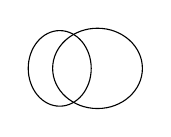
\begin{tikzpicture}[baseline=0cm]
\draw (0,0) ellipse (0.40cm and 0.48cm);
\draw (0.48,0) ellipse (0.57cm and 0.51cm);
\end{tikzpicture}
\quad $U\subset\mathbb H^n$, $V\subset\mathbb H^n$.
\begin{equation*}
f:U\to V.
\end{equation*}
\begin{equation*}
\forall x\in U\quad df_x:\mathbb H^n\to\mathbb H^n
\tag{1}
\end{equation*}
a morphism of left modules
([crossed out: \EnglishUnclear{GELFAND-P001371}{morphism-cancellation}{matr.? [source abbreviation]}]
multiplication by a matrix on the right).

If it is simply connected, only a linear space results.
[Beneath the line: an opening parenthesis with no continuation.]

All automorphisms are linear.

One can write the Lie algebra of infinitesimal transformations that preserve it.

(2) \underline{Assertion}: then the transition functions must be linear.

The first approximation is \EnglishUnclear{GELFAND-P001371}{approximation-ending}{trivial [uncertain abbreviated ending]?}.

A vector field whose differential is a quaternionic matrix
[crossed out: \EnglishUnclear{GELFAND-P001371}{matrix-cancellation}{an illegible sign}].

\underline{Definition (1) is incorrect}, since then projective space would not
have a quaternionic structure.

$\mathbb C P^n$ --- the space of 1-dimensional quaternionic subspaces in $\mathbb H^{n+1}$.

$\mathbb C P^1$ --- pairs $(\lambda_1,\lambda_2)$ up to left multiplication
$(\lambda\lambda_1,\lambda\lambda_2)$.
\EnglishUnclear{GELFAND-P001371}{projective-space-letter}{The letter $\mathbb C$ is visible in the projective-space notation.}

2 charts \quad $(\lambda_1,1)$,\quad $(1,\lambda_2)$.
\begin{equation*}
(\lambda_1,1)\sim(1,\lambda_1^{-1}).
\end{equation*}
$\lambda\to\lambda^{-1}$ --- the transition function.


\EnglishSourceFrame{GELFAND-P001372}{50}
$\lambda^{-1}$
\begin{equation*}
(\lambda_0+i\lambda_1+j\lambda_2+k\lambda_3)^{-1}
=\frac{\lambda_0-i\lambda_1-j\lambda_2-k\lambda_3}
{\lambda_0^2+\lambda_1^2+\lambda_2^2+\lambda_3^2}.
\end{equation*}
\begin{equation*}
d(\lambda^{-1})=-\lambda^{-1}d\lambda\,\lambda^{-1}.
\end{equation*}

\underline{Topological explanation}: if this were so, there would be 3 complex structures on $S^3$.

$V=\mathbb R^{4n}$.

(3) \underline{Quaternionic structure} --- a subalgebra $Q\subset$
[crossed out: \EnglishUnclear{GELFAND-P001372}{endomorphism-cancellation}{an illegible sign}]
$\operatorname{End}(V)$, isomorphic to $\mathbb H$.

(Or a subalgebra spanned by 3 anticommuting complex structures
\begin{equation*}
Q=\langle I,J,K,E\rangle,\qquad
I^2=J^2=K^2=-1,\quad IJ=-JI=K
\end{equation*}
and so on.

$\Rightarrow$ one can multiply by quaternions on the left.

\underline{Alternatively}: the isomorphism is not fixed; there is no need to single out $I$, $J$ and $K$.

($\mathbb H$ has nontrivial automorphisms.)

\underline{Quaternionic structure} on a manifold: a field of quaternionic structures
(in each tangent space). (Or: an almost quaternionic structure.)

Chern (1945) considered such structures.

($\forall$ 4-dimensional Riemannian manifold has two, since
$\operatorname{SO}(4)=\text{product}$

$M^{4n}$, $Q:x\mapsto Q_x$.

\underline{Integrability}: instead of an atlas, Cauchy--Riemann equations.

(Up to second-order infinitesimals
[crossed out: \EnglishUnclear{GELFAND-P001372}{integrability-cancellation}{an illegible word}]
as a quaternionic transformation)

\underline{Automorphisms preserving a quaternionic structure}
\begin{equation*}
G=\operatorname{GL}(1,\mathbb H)\cdot\operatorname{GL}(n,\mathbb H)
\qquad\text{--- the automorphism group of a quaternionic structure}
\end{equation*}
\begin{equation*}
G=\operatorname{Sp}(1)\cdot\operatorname{Sp}(n)
\end{equation*}
--- for [crossed out:
\EnglishUnclear{GELFAND-P001372}{sp-word-cancellation}{ordinary [source masculine ending]?}]
definition (1).
[Also crossed out above the cancelled word:
\EnglishUnclear{GELFAND-P001372}{sp-upper-cancellation}{an illegible sign}.]
\EnglishUnclear{GELFAND-P001372}{automorphism-groups}{The groups and the reference to definition (1) are reproduced literally.}

\begin{equation*}
y_i=\sum x_k a_{ki}
\end{equation*}
[Crossed out between $\sum$ and $x_k$:
\EnglishUnclear{GELFAND-P001372}{summation-cancellation}{an illegible symbol}.]
$\Vert$ preserves the quaternionic structure (right).
\EnglishUnclear{GELFAND-P001372}{right-structure}{The word "right" is preserved.}

\begin{equation*}
(x_1,\ldots,x_n)\to(\lambda x_1,\ldots,\lambda x_n)
\end{equation*}
also preserves it.

[Crossed out in the right-hand parentheses before the first $\lambda$:
\EnglishUnclear{GELFAND-P001372}{tuple-first-cancellation}{$x_1$?};
crossed out between this $\lambda$ and $x_1$:
\EnglishUnclear{GELFAND-P001372}{tuple-second-cancellation}{an illegible sign}.]

[Beneath the formula, with an arrow to the position between the first $\lambda$ and $x_1$:]
(On the other side!)


\EnglishSourceFrame{GELFAND-P001373}{unlabelled}
\underline{Condition for 1-integrability:}

$\exists$ a torsion-free connection $\nabla$ preserving the quaternionic structure.

(A linear connection, not necessarily a metric connection.)

[Crossed out in parentheses:
\EnglishUnclear{GELFAND-P001373}{cancelled-parenthesis}{an illegible phrase}.]
Or: $\nabla Q=0$.

Quaternionic subspace $\longrightarrow$ quaternionic subspace under parallel transport.

[Separator stroke.]

\underline{Goncharov A.}

Let there be a real-analytic manifold with an [inserted: almost] quaternionic structure.
\begin{equation*}
M_{\mathbb R}^{4n}\subset M_{\mathbb C}^{4n}.
\end{equation*}
\begin{equation*}
T_xM_{\mathbb C}^{4n}\supset K_x
=\bigcup\{v+\sqrt{-1}\,Jv\},\qquad v\in TM_{\mathbb R}^{4n},
\end{equation*}
[Above $K_x$: cone.]
\begin{equation*}
J\in Q_x,\qquad J^2=-1.
\end{equation*}
And there must be integrability.

[Separator stroke.]

D. A.
\begin{equation*}
\gamma\text{ --- a curve}\quad\Rightarrow\quad
\tau_\gamma Q_{\gamma(0)}=Q_{\gamma(1)}.
\end{equation*}
\begin{equation*}
\gamma:[0,1]\to M.
\end{equation*}
($\tau_\gamma$ --- parallel transport along $\gamma$.)

$Q_x$ --- a subalgebra in $\operatorname{Aut}T_xM$;
it can also be transported.
\EnglishUnclear{GELFAND-P001373}{algebra-in-aut}{The manuscript reads "a subalgebra in $\operatorname{Aut}T_xM$".}


\EnglishSourceFrame{GELFAND-P001374}{unlabelled}
\underline{20/IV-87}\qquad\underline{Gelfand seminar.}

\underline{I. M. G.} Question: there are 2 commuting isometries in an $n$-dimensional space;
[Addition above the line with a pointer: not defined everywhere.]
how can one turn them into 2 commuting unitary operators? What are the obstructions?

This has been done in part by Kasparov.

\underline{Kirillov on Jones's work.}

\underline{Distinguishing}
[crossed out: \EnglishUnclear{GELFAND-P001374}{knot-cancellation}{knots?}]
\underline{knots using factors.}

Consider the algebra generated by the generators $T_i$ (infinitely many) with the relations
\begin{equation*}
\begin{cases}
(T_i+1)(T_i-q)=0,\\
T_iT_{i+1}T_i=T_{i+1}T_iT_{i+1},\\
T_iT_j=T_jT_i,\quad |i-j|>1.
\end{cases}
\tag{1}
\end{equation*}
(The Hecke algebra of series $A$.)

$\Rightarrow$ [crossed out:
\EnglishUnclear{GELFAND-P001374}{series-cancellation}{an illegible sign}]
in Leningrad they \EnglishUnclear{GELFAND-P001374}{leningrad-verb}{applied [uncertain source verb]?}
also series $B$.

1. Knot $\longrightarrow$ polynomial; equivalent knots $\longrightarrow$ equal polynomials.

2. Factor $\longrightarrow$ subfactor.


\EnglishSourceFrame{GELFAND-P001375}{unlabelled}
Consider $\coprod_n B_n$
([crossed out: \EnglishUnclear{GELFAND-P001375}{union-cancellation}{an illegible abbreviation}]
disjoint union).
[Beneath $B_n$ with a pointer: braid group.]

\underline{Link}: an oriented 1-dimensional compact manifold immersed in $\mathbb R^3$.
\EnglishUnclear{GELFAND-P001375}{link-immersion}{The definition says "immersed".}

[To the left of the diagram: \EnglishUnclear{GELFAND-P001375}{left-isolated-mark}{a short isolated stroke}.]

\EnglishSourceFigure{GELFAND-P001375}{braids-links-diagram}{At the top, $\coprod_n B_n$.
From it an arrow points down-left to $H$, and an arrow points right-down to a drawing of two
overlapping oriented loops. To the left of $H$ is "factor";
beneath $H$, with a short pointer, is "Hecke algebra (1)".
From $H$ an arrow points down-right to the word "polynomials".
In the loop drawing both visible arrows point upwards along the right branches;
the upper arcs are faint and interrupted, and the connections and upper crossing require checking against the scan.}

% Future-only, uncompiled partial ink recreation; no live frame replacement.
% P1375 original native diagram bbox [185,450,1445,960].
% Coordinates below are original scan pixels; Bézier centerlines are approximate.
% The topological connectivity and over/under order are intentionally unresolved.
% Existing frame prose and its seven literal Unclear calls are outside this fragment.
\EnglishReaderDiagramPair{figures/gelfand-0149-p001375-braids-links-original.png}{GELFAND-P001375}{%
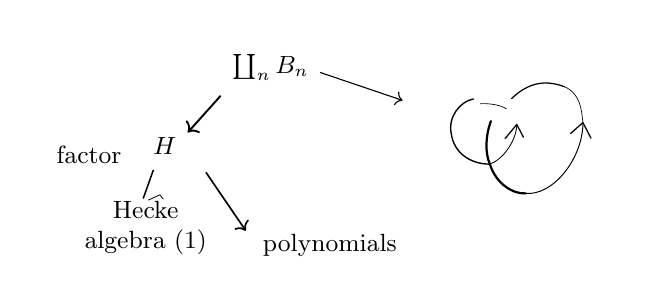
\begin{tikzpicture}[x=0.006cm,y=-0.006cm,line cap=round,line join=round,
  every node/.style={inner sep=1pt,font=\small}]
\path[use as bounding box] (185,450) rectangle (1445,960);
\node at (700,535) {$\coprod_n B_n$};
\node at (475,700) {$H$};
\node at (315,720) {factor};
\node[align=center] at (435,874) {Hecke\\algebra $(1)$};
\node at (825,910) {polynomials};
% Three directly visible directed connecting strokes.
\draw[->,line width=0.7pt] (593,595) -- (524,672);
\draw[->,line width=0.4pt] (805,545) -- (979,604);
\draw[->,line width=0.6pt] (563,757) -- (647,880);
% The lower-left shaft and separate bent stroke are kept separate.
% Neither a new arrowhead nor a reverse-directed arrow is inferred here.
\draw[line width=0.55pt] (451,752) -- (430,811);
\draw[line width=0.3pt] (441,815) -- (465,804) -- (472,813);
% Left visible curved strand: open at the upper left and at its right arrowhead.
\draw[line width=0.5pt] (1129,601)
  .. controls (1101,606) and (1075,639) .. (1082,674)
  .. controls (1088,716) and (1123,739) .. (1164,739);
\draw[line width=0.3pt] (1164,739)
  .. controls (1190,730) and (1219,692) .. (1221,657);
% Detached faint upper fragment, preserving the native visible gap.
\draw[line width=0.25pt] (1144,611)
  .. controls (1160,610) and (1186,613) .. (1199,622);
% A separate explicit visible upward arrowhead, with no inferred upper closure.
\draw[line width=0.45pt] (1196,685) -- (1221,655) -- (1235,682);
% Right visible curved strand: inner upper endpoint remains open.
% Its lower contact with the left curve is drawn without a vertex or underpass.
\draw[line width=0.8pt] (1166,648)
  .. controls (1155,677) and (1153,715) .. (1164,739)
  .. controls (1177,782) and (1215,803) .. (1240,801);
\draw[line width=0.35pt] (1240,801)
  .. controls (1298,806) and (1359,728) .. (1361,655);
% Separate upper arc; do not connect its left endpoint to the inner strand.
\draw[line width=0.45pt] (1210,600)
  .. controls (1250,562) and (1286,562) .. (1322,575);
\draw[line width=0.25pt] (1322,575)
  .. controls (1356,590) and (1358,624) .. (1361,651);
\draw[line width=0.45pt] (1335,674) -- (1361,651) -- (1378,684);
\end{tikzpicture}
}
\EnglishUnclear{GELFAND-P001375}{braids-links-connectivity}{The upper gaps in the two curves are left open as visible in the drawing; their connections and the over/under order at the lower contact are not established.}
\EnglishUnclear{GELFAND-P001375}{hecke-indicator}{Beneath $H$ there is a slanting stroke and a separate angled stroke above the caption ``Hecke algebra (1)''; a definite arrowhead and indicator direction are not established.}


Braid $\longrightarrow$ link (join the beginning to the end).

Identity braid $\longrightarrow$
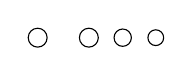
\begin{tikzpicture}[baseline=-0.1cm]
\draw (0,0) circle (0.12cm);
\draw (0.65,0) circle (0.12cm);
\draw (1.08,0) circle (0.11cm);
\draw (1.50,0) circle (0.10cm);
\end{tikzpicture}

(2) $b\subset B_n$ and $\widetilde b\subset B_n$ define equivalent links.
[Beneath $\widetilde b$:] $\widetilde b=cbc^{-1}$.
[On the right, beyond a vertical stroke:] $B_n\subset B_{n+1}$.
\EnglishUnclear{GELFAND-P001375}{braid-membership}{In (2), the signs before $B_n$ resemble $\subset$.}

(3) $b\in B_n$, $\widetilde b\in B_{n+1}$,
$\widetilde b=b\cdot\sigma_n^{\pm1}$
(appending one generator from $B_{n+1}$).

Then $b$ and $\widetilde b$ generate
[crossed out: \EnglishUnclear{GELFAND-P001375}{equivalence-cancellation}{equiv.? [source abbreviation]}]
equivalent links.

% Source diagram: bbox [385,1760,705,2150], original pixels.
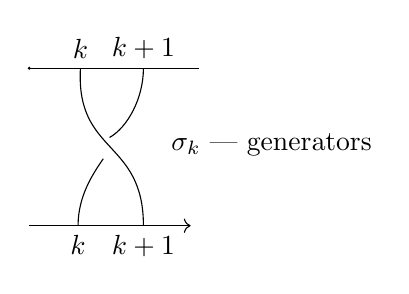
\begin{tikzpicture}[baseline=0cm]
\draw (-0.65,2) -- (1.50,2);
\fill (-0.65,2) circle (0.02cm);
\draw[->] (-0.65,0) -- (1.40,0);
\draw (0.80,2) .. controls (0.80,1.62) and (0.60,1.25) .. (0.37,1.12);
\draw (-0.03,0) .. controls (-0.03,0.38) and (0.16,0.66) .. (0.29,0.85);
\draw (0,2) .. controls (-0.06,0.90) and (0.80,1.10) .. (0.80,0);
\node[above] at (0,2) {$k$};
\node[above] at (0.80,2) {$k+1$};
\node[below] at (-0.03,0) {$k$};
\node[below] at (0.80,0) {$k+1$};
\node[right] at (1.03,1.03) {$\sigma_k$ --- generators};
\end{tikzpicture}

(4) \underline{Markov's theorem} (difficult): the described operations suffice
to pass to any equivalent link.

Idea: construct a function invariant under these operations.

The map from $\coprod_n B_n$ to $H$ is constructed as follows:
$\sigma_i\to T_i$, $\sigma_i^{-1}\to T_i^{-1}$.
[Beneath $T_i^{-1}$: found from the quadratic equation $(1)_1$.]

$(1)_{2,3}$ --- a complete set of relations in the braid group.
\begin{equation*}
\sigma_i^{-1}\longrightarrow\frac{T_i+(1-q)}{q}=T_i^{-1}.
\end{equation*}

The set of generators (1) [inserted: $\forall q$] has a unique factor representation
with a trace, and
[crossed out: \EnglishUnclear{GELFAND-P001375}{trace-cancellation}{an illegible fragment}]
the trace is a polynomial in $q$, $q^{-1}$.
\begin{equation*}
\mathbb Z[q,q^{-1}].
\end{equation*}
\EnglishUnclear{GELFAND-P001375}{factor-claim-parameter}{The addition $\forall q$ and the uniqueness assertion are left without supplementation.}


\EnglishSourceFrame{GELFAND-P001376}{57}
\underline{Exercise}. Take $q=\pm1$ and see which invariant
of the braid group results here (the ratio of the values of
Jones's polynomial at these values).

\underline{Jones} specifically excluded from consideration
[crossed out: \EnglishUnclear{GELFAND-P001376}{roots-cancellation}{an illegible fragment}]
roots of $1$.

\underline{Idea of I. M. G.}: consider precisely roots of $1$.
It may turn out that there are no factors at all and that what is needed is roots of $1$.

A. M. Vershik has already done something on this subject.

\paragraph*{\underline{A. Beilinson.}}
On work by Beilinson, MacPherson and V. Schechtman.

\underline{Notes on motivic cohomology}

Let $X$ be an analytic manifold and $E$ a vector bundle on $X$.
[Beneath the description of $X$:] (or \EnglishUnclear{GELFAND-P001376}{x-parenthesis}{complex [source abbreviation]?})
(compact).
\begin{equation*}
c_i(E)\in H^{2i}(X,\mathbb C)
=H^{2i}(X,\mathcal O\to\Omega^1\to\ldots).
\end{equation*}
[Above the last argument, with a pointer: cohomology with coefficients in a complex of sheaves.]

They are integral and satisfy the Hodge condition
([crossed out: \EnglishUnclear{GELFAND-P001376}{hodge-cancellation}{an illegible word}]
$c_i\in i$-th term of the Hodge filtration).

(Since they can be computed using $\log$ of products in Cech cocycles.)

Compute the cohomology of the manifold from the de Rham complex.
\begin{equation*}
(1)\qquad 0\to\mathbb C\to
\text{[crossed out: }\EnglishUnclear{GELFAND-P001376}{de-rham-cancellation}{an illegible sign}\text{]}
\mathcal O\to\Omega^1\to\Omega^2\to\ldots
\end{equation*}
[On the right:] $\Omega^i$ --- holomorphic $i$-forms (a sheaf).

$\{U_i\}$ --- a covering of $X$ by small open sets.

Associate:
\begin{center}
$(*)\quad$
\begin{tikzcd}
C^{2i}(\mathcal O)\arrow[r] & C^{2i}(\Omega^1) \\
 & C^{2i-1}(\Omega^1)\arrow[u]\arrow[r] & \ldots
\end{tikzcd}
\end{center}

The Hodge filtration on $H^k(X,\mathbb C)$:
\begin{equation*}
F^j H^k(X,\mathbb C)
=H^k(X,0\to\ldots\to0\to\Omega^j\to\Omega^{j+1}\to\ldots).
\end{equation*}
\underline{Atiyah's construction of a characteristic class, from which it follows that $c_j\in F^j$}.

$g_{ij}$ --- transition functions.
\begin{equation*}
g_{ij}\colon U_i\cap U_j\longrightarrow GL_n(\mathbb C).
\end{equation*}
\begin{equation*}
A=g_{ij}^{-1}dg_{ij}\in
\Omega^1(U_i\cap U_j,\operatorname{Mat}_n(\mathbb C))
\in C^1(X,\Omega^1\otimes\operatorname{Mat}_n).
\end{equation*}
[Beneath $g_{ij}^{-1}dg_{ij}$: a 1-form with values in a Lie algebra.]
\EnglishUnclear{GELFAND-P001376}{cochain-membership}{The formula for $A$ retains two successive $\in$ signs.}

Take $(g_{ij}^{-1}dg_{ij})^k$ --- a cochain with values in $k$-forms.
[Beneath the power: (multiplication of cochains; the closing parenthesis is not visible. On the right, a double stroke.]

Take the trace $\operatorname{Tr}$ $\longrightarrow$ a form with one component is obtained.


\EnglishSourceFrame{GELFAND-P001377}{unlabelled}
\begin{equation*}
c_i(E)=\operatorname{Tr}(A^i).
\end{equation*}
[On the right:] $A^i$ --- a form of degree $i$ on the intersection of the $(i+1)$-st set.
\EnglishUnclear{GELFAND-P001377}{chern-trace}{The notation $c_i(E)$ before the trace of the power is preserved.}

[Crossed out: \EnglishUnclear{GELFAND-P001377}{element-cancellation}{Vid? [unresolved source fragment]}]
$\Rightarrow$ an element of $2i$-dimensional cohomology (see diagram $(*)$).

\underline{Problem}: explicitly construct a homotopy into an integral characteristic class.

For
\begin{equation*}
c_1=d\log(\det g_{ij}).
\end{equation*}

Drop $d$:
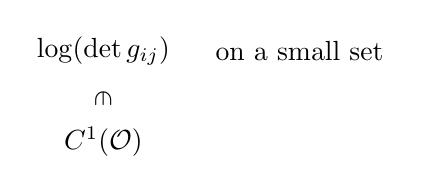
\begin{tikzpicture}[baseline=0cm]
\node at (0,0) {$\log(\det g_{ij})$};
\node[right] at (1.3,0) {on a small set};
\node[rotate=-90] at (0,-0.60) {$\in$};
\node at (0,-1.15) {$C^1(\mathcal O)$};
\end{tikzpicture}


\EnglishSourceFrame{GELFAND-P001378}{unlabelled}
\underline{27.4.87}\qquad \underline{Gelfand seminar}

\paragraph*{\underline{A. Beilinson}}
\underline{Deligne cohomology} [inserted above the end of the heading: --- Beilinson]:
see \EnglishUnclear{GELFAND-P001378}{soule-reference}{survey [source abbreviation]?} Soulé,
Bourbaki seminar, Feb. 85.
[Beneath the surname:] (Regulateurs).

\underline{H. Esnault, E. Viehweg} (preprint).
[Beneath "preprint": Manin has a copy.]

Deligne--Beilinson cohomology

\underline{Beilinson}: Modern Problems in Mathematics, vol. 24.

Contempor. math. \EnglishUnclear{GELFAND-P001378}{bibliography-number}{$\sim$ No. 25?}

\underline{Complex of sheaves} on any manifold (complex analytic schemes).
\begin{equation*}
(1)\qquad
\mathbb Z(i)_{\mathcal D}:=
\mathbb Z\overset{(2\pi\sqrt{-1})^i}{\longrightarrow}
\mathcal O\longrightarrow\Omega^1\longrightarrow\ldots
\longrightarrow\Omega^{i-1}.
\end{equation*}

($i$ is an integer.)

In particular
\begin{equation*}
\mathbb Z(0)_{\mathcal D}=\mathbb Z,
\end{equation*}
\begin{equation*}
\mathbb Z(1)_{\mathcal D}=
\bigl(\mathbb Z\overset{2\pi\sqrt{-1}}{\longrightarrow}\mathcal O\bigr)
\overset{\exp}{\longrightarrow}\mathcal O^*[-1].
\end{equation*}
[Beneath $\mathcal O^*$, a bracket with the caption: degree 1.]

[On the right:]
\begin{tikzcd}
\mathbb Z\arrow[r]\arrow[d] & \mathcal O\arrow[d,"\exp"] \\
0\arrow[r] & \mathcal O^*
\end{tikzcd}

[Beneath the diagram:] a morphism of complexes.

The cohomology sheaf is
\begin{equation*}
H^1(\mathbb Z(1))=\mathcal O^*.
\end{equation*}
\begin{equation*}
\mathbb Z(2)_{\mathcal D}=
\bigl(\mathbb Z\overset{-4\pi^2}{\longrightarrow}\mathcal O
\longrightarrow\Omega^1\bigr).
\end{equation*}
\begin{equation*}
H^1(\mathbb Z(2)_{\mathcal D})=
\mathbb C/(2\pi\sqrt{-1})^2\mathbb Z.
\end{equation*}
[Beneath the right-hand side:]
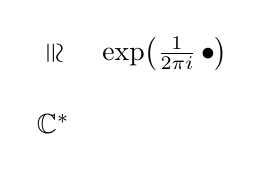
\begin{tikzpicture}[baseline=0cm]
\node[rotate=-90] at (0,0) {$\cong$};
\node[right] at (0.5,0) {$\exp\bigl(\frac{1}{2\pi i}\,\bullet\bigr)$};
\node at (0,-0.9) {$\mathbb C^*$};
\end{tikzpicture}
\EnglishUnclear{GELFAND-P001378}{exponential-placeholder}{The final sign in the exponent argument resembles a dot or a circle.}

\begin{equation*}
H^2(\mathbb Z(2)_{\mathcal D})=\Omega^1/d\mathcal O.
\end{equation*}

\EnglishSourceFrame{GELFAND-P001379}{67}
there is a map
\begin{equation*}
\mathbb{Z}(i)_{\mathcal D}\longrightarrow\mathbb{Z}
\qquad\text{(zeroth component)}\tag{2}
\end{equation*}
\begin{equation*}
\mathbb{Z}(i)_{\mathcal D}\longrightarrow\Omega^i[-i]\tag{3}
\end{equation*}
(0 on all forms; the last is sent to its differential)
\begin{equation*}
\mathbb{Z}(i)_{\mathcal D}\otimes\mathbb{Z}(j)_{\mathcal D}
\longrightarrow\mathbb{Z}(i+j)_{\mathcal D}\tag{4}
\end{equation*}
\begin{equation*}
z_i\star\omega_j=z_i\omega_j
\end{equation*}
[To the right of (4):] the arrows (2) and (3) take this multiplication to ordinary multiplication of numbers and forms.

Let $z_j$ be from the zeroth component.
\begin{equation*}
z_1\star z_2=z_1z_2\qquad\text{(ordinary product)}\tag{5'}
\end{equation*}
\begin{equation*}
z_1\star\omega_2=z_1\omega_2\tag{5''}
\end{equation*}
\begin{equation*}
\omega_1\star z_2=z_2\omega_1\tag{5'''}
\end{equation*}
\begin{equation*}
\omega_1\star\omega_2=
\begin{cases}
0, & \text{if }\omega_2\notin\Omega^{j-1},\\
\omega_1\wedge d\omega_2, & \text{if }\omega_2\in\Omega^{j-1}
\end{cases}\tag{6}
\end{equation*}
(7) Up to \underline{homotopy}, this multiplication is commutative.
[Beneath "homotopy": (of chain complexes).]

(8) Both maps (2), (3) commute with multiplication.

(9) Let $E$ be a holomorphic vector bundle [inserted: on $X$]. Its Chern classes are then defined
\begin{equation*}
c_i(E)\in H^{2i}(X,\mathbb{Z}(i)_{\mathcal D})
\end{equation*}
[On the right:] (cohomology group with coefficients in a complex of sheaves).
[Added above the beginning of the note:
\EnglishUnclear{GELFAND-P001379}{eq09-insertion}{abelian [source inflection uncertain]}.]

(10) Under the map (2), they become the usual topological Chern classes;
this property and functoriality determine the classes (9) uniquely.

\underline{Description of the group} $H^{2i}(X,\mathbb{Z}(i)_{\mathcal D})$.

Let $X$ be compact.

The Cech definition of cohomology in (9).

$C^{ij}$ denotes $i$-dimensional cochains with coefficients in the $j$th sheaf.

[Crossed out to the left of the diagram:
\EnglishUnclear{GELFAND-P001379}{cochain-cancellation}{an illegible sign}.]
\begin{equation*}
\begin{tikzcd}[column sep=large,row sep=large]
C^{ij}\arrow[r,"d"]\arrow[dr,"\delta"'] & C^{i,j+1}\\
& C^{i+1,j}
\end{tikzcd}
\end{equation*}
[On the right:] $d$ is the differential in the complex (de Rham).

Now, for $d+\delta$, we have ordinary cohomology.

(This is obtained for $C^*$ [crossed out:
\EnglishUnclear{GELFAND-P001379}{bottom-cancellation}{an illegible sign}]
$X$ (integer-valued)).


\EnglishSourceFrame{GELFAND-P001380}{unlabelled}
For compact $X$
\begin{equation*}
H^n(X,\mathbb{C})=\bigoplus_{a+b=n}H^{a,b}(X)
\qquad\text{(Hodge decomposition)}\tag{11}
\end{equation*}
\begin{equation*}
F^iH^n(X,\mathbb{C})=\bigoplus_{a\ge i}H^{a,b}
\qquad\text{(Hodge filtration)}\tag{12}
\end{equation*}
It is known that
\begin{equation*}
H^{a,b}(X)=H^b(X,\Omega^a)\tag{13}
\end{equation*}
Then
\begin{equation*}
\begin{gathered}
0\longrightarrow
\frac{H^{n-1}(X,\mathbb{C})}
{H^{n-1}(X,\mathbb{Z})+F^iH^{n-1}(X,\mathbb{C})}
\longrightarrow H^n\bigl(X,\mathbb{Z}(i)_{\mathcal D}\bigr)\\
\longrightarrow H^n(X,\mathbb{Z})\cap F^iH^n(X,\mathbb{C})\longrightarrow0
\end{gathered}\tag{14}
\end{equation*}
[Crossed out in the middle term of (14), after $X,$ and before $\mathbb Z(i)_{\mathcal D}$:
\EnglishUnclear{GELFAND-P001380}{eq14-cancellation}{an illegible sign}.]
A Deligne cohomology class $\sim$ (the difference between an integer-valued cocycle and a de Rham cocycle) $+$ (a homotopy connecting them).

\underline{A cochain with coefficients in the Deligne complex.}

A cocycle $\alpha$ [a lower sign is crossed out or corrected:
\EnglishUnclear{GELFAND-P001380}{cocycle-index}{illegible}]
$\in Z^n(X;\mathbb{Z}(i)_{\mathcal D})$ consists of a collection
\begin{equation*}
\begin{cases}
\alpha_0\in Z^n(X,\mathbb{Z}),\\
\alpha_1\in C^{n-1}(X,\mathcal O),\\
\alpha_2\in C^{n-2}(X,\Omega^1),\\
\vdots\\
\alpha_i\in C^{n-i}(X,\Omega^{i-1}),
\end{cases}\tag{15}
\end{equation*}
compatible in the sense that
\begin{equation*}
\begin{cases}
\alpha_0=\delta\alpha_1,\\
d\alpha_1=\delta\alpha_2,\\
\vdots\\
\delta\alpha_i=d\alpha_{i-1}
\end{cases}\tag{16}
\end{equation*}
Hence
\begin{equation*}
d\alpha_i\in Z^{n-i}(X,\Omega^{i,\mathrm{cl}})
\qquad\text{(with values in closed forms)}\tag{17}
\end{equation*}
Therefore one may consider
\begin{equation*}
\alpha_0-d\alpha_i\in Z^n(X,\Omega^\bullet)\tag{18}
\end{equation*}
(The rest is a homotopy, \EnglishUnclear{GELFAND-P001380}{bottom-abbreviation}{ustanavl. [unexpanded Russian abbreviation]}


\EnglishSourceFrame{GELFAND-P001381}{unlabelled}
[Number at the upper right: \EnglishUnclear{GELFAND-P001381}{page-label}{68 / 62}.]

$\alpha_1+\alpha_2+\ldots+\alpha_i$
[crossed out: \EnglishUnclear{GELFAND-P001381}{top-cancellation}{illegible}]
$\in C$.
\begin{equation*}
d(\alpha_0+\alpha_1+\ldots+\alpha_i)=\alpha_0-d\alpha_i\tag{19}
\end{equation*}
\EnglishUnclear{GELFAND-P001381}{eq19-first-index}{In the parentheses, the first subscript reads as $0$; in the line above, the sum begins with $\alpha_1$.}

So far, these are general facts in every double complex [source symbol: $\forall$].

(see also the work of Gabrielov, Gelfand and Losik)

Describe the group $H^{2i}(X,\mathbb{Z}(i)_{\mathcal D})$ starting from (14).
\begin{equation*}
\begin{gathered}
0\longrightarrow
\underbrace{\frac{H^{2i-1}(X,\mathbb C)}{H^{2i-1}(X,\mathbb Z)+F^i}}_{\substack{\Vert\\ J^i}}
\longrightarrow H^{2i}(X,\mathbb Z(i)_{\mathcal D})\\
\longrightarrow
\underbrace{H^{2i}(X,\mathbb Z)\cap F^iH^{2i}(X,\mathbb C)}_{\substack{\Vert\\ \mathrm{Hg}^i(X,\mathbb Z)}}
\longrightarrow0
\end{gathered}\tag{20}
\end{equation*}
[Beneath $J^i$:] (a complex torus called the $i$th Griffiths Jacobian).
\begin{equation*}
H^{2i-1}=F^i\oplus\overline F^{\,i}
\end{equation*}
$\Rightarrow$ this gives the complex structure on $J^i$.

(21) \underline{Example.}
\begin{equation*}
c_1(\mathcal E)=c_1(\det\mathcal E)
\end{equation*}
$g_{ij}$ are the transition functions of the bundle
[crossed out: \EnglishUnclear{GELFAND-P001381}{transition-cancellation}{an illegible sign before $\mathcal E$}]
$\mathcal E$

(with values in $\mathbb C^*$).
\begin{equation*}
c_1(\mathcal E)\in H^2(X,\mathbb Z(1)_{\mathcal D})
\end{equation*}
\begin{equation*}
c_1(\mathcal E)_0\in Z^2(X,\mathbb Z)\tag{22}
\end{equation*}
[In (22), a lower sign at $\mathcal E$, before the closing parenthesis, is crossed out or corrected:
\EnglishUnclear{GELFAND-P001381}{eq22-correction}{illegible}.]
\begin{equation*}
c_1(\mathcal E)_1\in C^1(X,\mathcal O),\tag{23}
\end{equation*}
where
\begin{equation*}
\delta[c_1(\mathcal E)_1]=c_1(\mathcal E)_0\tag{23'}
\end{equation*}
(24) $c_1(\mathcal E)_1=$
\EnglishUnclear{GELFAND-P001381}{eq24-factor}{$\log(\operatorname{deg}g_{ij})$ / $\log(\det g_{ij})$}
--- any determination of $\log$.

($c_1(\mathcal E)_0$ is found from (23')
[crossed out: \EnglishUnclear{GELFAND-P001381}{eq24-comment-cancellation}{an illegible sign}]
and gives the discrepancy).

An isomorphism is obtained
\begin{equation*}
c_1:\operatorname{Pic}(X)\overset{\sim}{\longrightarrow}H^2(X,\mathbb Z(1)_{\mathcal D})\tag{25}
\end{equation*}


\EnglishSourceFrame{GELFAND-P001382}{unlabelled}
\underline{Construction of $c_2$} (this is already related to the dilogarithm).

$c_1$ was constructed in two steps
\begin{equation*}
\mathcal E\overset{\det}{\longmapsto}
c_{1\,\mathrm{alg}}(\mathcal E)\in H^1(X,\mathcal O^*)
\overset{\text{«}\log\text{»}}{\longrightarrow}
H^2(X,\mathbb Z(1)_{\mathcal D})\tag{26}
\end{equation*}
In principle, one should have
\begin{equation*}
\begin{gathered}
c_i:\mathcal E\longmapsto
\underset{\substack{\Vert\\c_{iM}(\mathcal E)\\\text{(motivic)}}}{c_{i\,\mathrm{alg}}(\mathcal E)}
=H^{2i}(X,\mathbb Z(i)_M)\\
\underset{\substack{\uparrow\\\text{polylogarithm}}}{\overset{\mathcal L i_i}{\longrightarrow}}
H^{2i}(X,\mathbb Z(i)_{\mathcal D})
\end{gathered}\tag{27}
\end{equation*}
\EnglishUnclear{GELFAND-P001382}{eq27-equality}{Between $c_{i\,\mathrm{alg}}(\mathcal E)$ and $H^{2i}$, the source has $=$.}

This theory exists up to torsion.

[Crossed out: \EnglishUnclear{GELFAND-P001382}{before-vnei-cancellation}{illegible}.]
in it $\mathbb Z(1)_M=\mathcal O^*[-1]$.

\underline{Several requirements.}

(28) a) $\mathbb Z(\text{negative number})_M=0$

b) $\mathbb Z(0)_M=\mathbb Z$

c) $\mathbb Z(1)_M=\mathcal O^*[-1]$

d)
\begin{equation*}
\mathbb Z(2)_M=(\mathbb Z(2)_M^1\longrightarrow
\underset{\substack{\Vert\\\wedge^2(\mathcal O^*)}}{\mathbb Z(2)_M^2}
\qquad\text{(up to 2-torsion)}
\end{equation*}
\EnglishUnclear{GELFAND-P001382}{eq28-parenthesis}{After the second term, the outer closing parenthesis is not visible.}
\begin{equation*}
i\ge1:\ H^j(\mathbb Z(i)_M)=0\quad\text{for }j\notin[1,i]\tag{29}
\end{equation*}
\begin{equation*}
H^i(\mathbb Z(i)_M)=\mathcal K_i^{\mathrm{Milnor}}
\qquad\text{(sheaf of Milnor $K$-functors)}\tag{30}
\end{equation*}
\underline{Milnor $K$-functor.}

For a smooth (algebraic) manifold, these are sheaves.

(31) a) $\mathcal K_0^{\mathrm{Mil}}=\mathbb Z$,

b) $\mathcal K_1^{\mathrm{Mil}}=\mathcal O^*$.

c) [In the left margin: (Steinberg relations).]
let $t\in\mathcal O^*$ and $1-t\in\mathcal O^*$; then
\begin{equation*}
\overset{\substack{\text{Steinberg symbol}\\\swarrow}}
{\underbrace{\{t,1-t\}}_{\text{product in the Milnor algebra}}}=0
\end{equation*}
\EnglishUnclear{GELFAND-P001382}{milnor-degree}{$\mathcal K_0^{\mathrm{Mil}}$ / $\mathcal K_\circ^{\mathrm{Mil}}$ / $\mathcal K_\bullet^{\mathrm{Mil}}$}
$=$ the free graded algebra with generators
[crossed out: $\mathcal O^*$]
$\mathcal O^*=\mathcal K_1^{\mathrm{Mil}}$ and Steinberg relations.

$\{ab,c\}=$ [crossed out:
\EnglishUnclear{GELFAND-P001382}{bottom-product-cancellation}{$\{a,c\}\{b,c\}$ / $\{a,c\}+\{b,c\}$}]
$?$.

[On the right:] $\{\ \}$ is addition.


\EnglishSourceFrame{GELFAND-P001383}{69}
(32) The operation $\{\ \}$ is supercommutative in $\mathcal K^{\mathrm{Mil}}$.

In (28) d)

[A number is crossed out in the left margin: \EnglishUnclear{GELFAND-P001383}{cancelled-number}{(33)?}.]
[The entire line is crossed out:
$\mathbb Z(2)_M^1=\mathbb Z[\mathbb P^1(X)]$.]
\begin{equation*}
\mathbb Z(2)_M^1=
\mathbb Z[(\mathbb P^1\setminus\{0,1,\infty\})(X)]/(\text{relations})
\tag{33}
\end{equation*}
[A line runs downward from the expression with $\mathbb P^1$ to the annotation:]
the sheaf of functions on $X$ that do not take the values $0,1,\infty$.

Differential:
\begin{equation*}
\begin{aligned}
\mathbb Z(2)_M^1&\longrightarrow\mathbb Z(2)_M^2\\
t&\longmapsto t\wedge(1-t)
\end{aligned}\tag{34}
\end{equation*}
The relation comes from the consideration that it lies in the kernel of the Steinberg symbol.

(five-term relation for the dilogarithm)

Let $f,g$ be two functions that are nowhere equal to one another and do not take the values $0,1,\infty$.
\begin{equation*}
(f,g,0,1,\infty)\tag{35}
\end{equation*}
(36) \underline{five distinct points on} $\mathbb P^1$;
\underline{omitting one at a time, we obtain five cross-}
\underline{ratios and must take their alternating}
\EnglishUnclear{GELFAND-P001383}{eq36-abbreviation}{f-yu [unexpanded Russian abbreviation]};
this is the five-term relation.

In place of this, one may take five independent functions.

(37) \underline{Assertion.} The relation (36) lies in the kernel of the differential.

First devised by Spencer and Bloch; Suslin established the connection with $K$-theory.

The complex is called the Bloch--Suslin complex.

One must construct a map
\begin{equation*}
\mathcal E\longmapsto c_2(\mathcal E)_M\in H^4(X,\mathbb Z(2)_M)\tag{38}
\end{equation*}
[Crossed out in (38), between $c_2(\mathcal E)_M$ and the sign $\in$:
\EnglishUnclear{GELFAND-P001383}{eq38-cancellation}{an illegible mathematical fragment}.]

and a function
\begin{equation*}
\mathbb Z(2)_M\longrightarrow\mathbb Z(2)_{\mathcal D}\tag{39}
\end{equation*}


\EnglishSourceFrame{GELFAND-P001384}{unlabelled}
Construct the map (39).

(40)
\begin{equation*}
\begin{tikzcd}[column sep=large,row sep=large]
&\mathbb Z(2)_M^1\arrow[r]\arrow[d,"\mathrm{dilog}"]
&\mathbb Z(2)_M^2\arrow[d]\\
\mathbb Z\arrow[r]&\mathcal O\arrow[r]&\Omega^1
\end{tikzcd}
\end{equation*}
[To the right of the diagram:]
\begin{center}
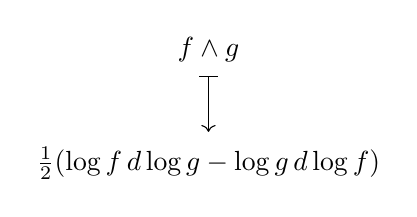
\begin{tikzpicture}
\node (upper) at (0,1.2) {$f\wedge g$};
\node (lower) at (0,-0.25) {$\frac12(\log f\,d\log g-\log g\,d\log f)$};
\draw[->] (0,0.85)--(0,0.15);
\draw (-0.12,0.85)--(0.12,0.85);
\end{tikzpicture}
\end{center}
\underline{Chern class.}
\begin{equation*}
\mathcal E\longmapsto c_2(\mathcal E)_M\in H^4(X,\mathbb Z(2)_M),\tag{41}
\end{equation*}
$\dim\mathcal E=2$, $\{U_i\}$, $s_i$ is a section of $\mathcal E$ over $U_i$.

Two components.
\begin{equation*}
c_2(\mathcal E)_M^2\in C^2(\{U_i\},\mathbb Z(2)_M^2)
\end{equation*}
\begin{equation*}
c_2(\mathcal E)_M^1\in C^3(\{U_i\},\mathbb Z(2)_M^1)
\end{equation*}
$(s_1,\ldots,s_4)$ are four sections of $\mathcal E$.

Consider four points $\mathbb P(\mathcal E)\ni s_1,\ldots,s_4$.

and so on

[Crossed out: \EnglishUnclear{GELFAND-P001384}{bottom-cancellation}{cross-ratio [abbreviated]}.]

It is constructed using the cross-ratio.


\clearpage\section*{Full reading notes}
The following records retain complete historical observations, candidates and source-review notes. Historical enlargement statements do not claim new decipherment. No uncertain reading is settled here.
\par

\subsection*{\texttt{GELFAND-P001359}}
\noindent\leavevmode\phantomsection\label{GELFAND-P001359:eq2-signs:note}\textbf{\texttt{GELFAND-0148-U001}} (eq2-signs).\par\nopagebreak[4]
Original PNG, region [470,750,1260,1200], coordinates measured from the upper left. In (1), the signs before 6uu\_x and u\_xxx are plus signs; (2) reads psi\_xx+u psi=k\textasciicircum{}2 psi and psi\_t=4 psi\_xxx+6u psi\_x+3u\_x psi. In (7), region [400,2320,1160,2480], the exponent is ikx+4ik\textasciicircum{}3t.\par
Candidates: The literal writing of (1), (2) and (7), with the visible plus signs. Unresolved in the diplomatic source.\par
For u=0, the function in (7) gives psi\_xx=-k\textasciicircum{}2 psi and psi\_t=+4ik\textasciicircum{}3 psi, whereas 4 psi\_xxx=-4ik\textasciicircum{}3 psi. This is an internal mathematical check, not a correction to the source. The sign contradiction is retained. Historical source review states that all regions were viewed again at 3x.\par\medskip
\noindent\leavevmode\phantomsection\label{GELFAND-P001359:eq3-overwriting:note}\textbf{\texttt{GELFAND-0148-U002}} (eq3-overwriting).\par\nopagebreak[4]
Original PNG, region [735,1365,1830,1545], coordinates measured from the upper left. In (3), the first K and following F are retraced or corrected with dense strokes. Between x and s, and between x and z, crossed-out plus signs have commas beneath them.\par
Candidates: Originally F beneath the final K and K beneath the final F; The original letters are illegible. Unresolved in the diplomatic source.\par
The final writing K(x,s,t)F(s+z,t) and K(x,z,t) is readable; the underlying letters have not been recovered. Historical source review states a repeated 4x view; an interchange of letters is not asserted.\par\medskip
\noindent\leavevmode\phantomsection\label{GELFAND-P001359:after-eq8-cancelled:note}\textbf{\texttt{GELFAND-0148-U003}} (after-eq8-cancelled).\par\nopagebreak[4]
Original PNG, region [590,2710,740,2840], coordinates measured from the upper left. After "we obtain" and before the dash, there is short densely crossed-out writing.\par
Candidates: psi; an illegible crossed-out symbol. Unresolved in the diplomatic source.\par
Historical source review states a 5x view of region [470,2690,795,2855]. The individual strokes do not permit confident recovery of the cancelled writing.\par\medskip

\subsection*{\texttt{GELFAND-P001360}}
\noindent\leavevmode\phantomsection\label{GELFAND-P001360:eq11-coefficient:note}\textbf{\texttt{GELFAND-0148-U004}} (eq11-coefficient).\par\nopagebreak[4]
Original PNG, region [775,575,885,700], coordinates measured from the upper left. Before the y derivative of psi in the first line of (11), a sign has a small upper loop and crossing lower strokes; it resembles both alpha and 2.\par
Candidates: alpha; 2. Unresolved in the diplomatic source.\par
Historical source review states a repeated 8x view. Alpha is readable in (10) and (12), making alpha contextually likely without resolving the graphical ambiguity in (11). The formula displays the candidate alpha with an explicit marker; this is not a correction.\par\medskip
\noindent\leavevmode\phantomsection\label{GELFAND-P001360:before-eq13-short-cancelled:note}\textbf{\texttt{GELFAND-0148-U005}} (before-eq13-short-cancelled).\par\nopagebreak[4]
Original PNG, region [1260,1480,1385,1570], coordinates measured from the upper left. Between "differently" and "understand", a short beginning of a word is crossed out.\par
Candidates: ob; op; illegible. Unresolved in the diplomatic source.\par
Historical source review states a 4x view in the broader region [350,1475,1510,1630]. The earlier writing has not been recovered.\par\medskip
\noindent\leavevmode\phantomsection\label{GELFAND-P001360:before-eq13-words-cancelled:note}\textbf{\texttt{GELFAND-0148-U006}} (before-eq13-words-cancelled).\par\nopagebreak[4]
Original PNG, region [355,1540,755,1630], coordinates measured from the upper left. Beneath the line beginning "However, one may...", two short words are crossed out. The second has a loop resembling the Cyrillic letter Ф and a descender.\par
Candidates: as Fourier; by Fourier; two illegible words. Unresolved in the diplomatic source.\par
Historical source review states a repeated 4x view. Both verbal candidates are conjectural; the crossed-out text has not been silently omitted.\par\medskip
\noindent\leavevmode\phantomsection\label{GELFAND-P001360:eq14-cancelled-argument:note}\textbf{\texttt{GELFAND-0148-U007}} (eq14-cancelled-argument).\par\nopagebreak[4]
Original PNG, region [1120,1990,1230,2160], coordinates measured from the upper left. In (14), between the arguments lambda-bar-prime and lambda, a cancelled symbol is crossed by several slanted strokes.\par
Candidates: lambda; chi; an illegible symbol. Unresolved in the diplomatic source.\par
Historical source review states a repeated 5x view of region [880,1920,1435,2160]. Analysis of the arguments of T does not recover the cancelled symbol; it is recorded separately from the final formula.\par\medskip
\noindent\leavevmode\phantomsection\label{GELFAND-P001360:eq15-overwritten-argument:note}\textbf{\texttt{GELFAND-0148-U008}} (eq15-overwritten-argument).\par\nopagebreak[4]
Original PNG, region [550,2320,620,2415], coordinates measured from the upper left. On the left-hand side of (15), the second argument of K is densely retraced. The final z is visible, with additional strokes beneath it.\par
Candidates: z over x; a retraced z. Unresolved in the diplomatic source.\par
Historical source review states a repeated 6x view of region [460,2300,665,2445]. The final z is preserved; the original writing is not asserted.\par\medskip

\subsection*{\texttt{GELFAND-P001361}}
\noindent\leavevmode\phantomsection\label{GELFAND-P001361:heading-ending:note}\textbf{\texttt{GELFAND-0148-U009}} (heading-ending).\par\nopagebreak[4]
Original PNG, region [1310, 525, 1545, 615], coordinates measured from the upper left. The last word of the underlined heading after d-bar has an ending in which the last stroke of ch is difficult to distinguish from an additional i.\par
Candidates: zadach.; zadachi.. Unresolved in the diplomatic source.\par
Historical source review states a repeated 4x view in [355,410,1555,640]. The grammatical preference for the plural is not treated as resolution of the graphical doubt.\par\medskip
\noindent\leavevmode\phantomsection\label{GELFAND-P001361:eq21-cancelled:note}\textbf{\texttt{GELFAND-0148-U010}} (eq21-cancelled).\par\nopagebreak[4]
Original PNG, region [385, 1870, 985, 2005], coordinates measured from the upper left. To the left of the final commutator (21), a commutator of two K entries with arguments lambda and eta, an equality sign and a final digit are crossed out. Strokes cross the subscripts.\par
Candidates: [K\_i(lambda),K\_i(eta)]=0; [K\_i(lambda),K\_j(eta)]=0. Unresolved in the diplomatic source.\par
Historical source review states a 5x view. In both K entries the clearest subscript resembles i; replacement of the second by j by analogy with the final formula is not asserted.\par\medskip
\noindent\leavevmode\phantomsection\label{GELFAND-P001361:time-coefficient:note}\textbf{\texttt{GELFAND-0148-U011}} (time-coefficient).\par\nopagebreak[4]
Original PNG, region [625, 1075, 1010, 1220], coordinates measured from the upper left. The third line of (19) visibly has the coefficient -4 without i. The same occurs in the exponent (20), region [1510,1310,1810,1450], and in I\_3=4 lambda\textasciicircum{}3 in (23), region [1135,2400,1420,2530].\par
Candidates: -4(lambda\textasciicircum{}3-eta\textasciicircum{}3) in (19),(20); I\_3=4 lambda\textasciicircum{}3 in (23). Unresolved in the diplomatic source.\par
Historical source review states that all three regions were viewed at 3x. Formulas (19),(20),(22),(23) agree with one another, but the connection of the time normalization to (7),(14) and the claimed KP equation (12) requires separate checking. No factor i was added from mathematical expectation.\par\medskip
\noindent\leavevmode\phantomsection\label{GELFAND-P001361:eq24-cancelled-argument:note}\textbf{\texttt{GELFAND-0148-U012}} (eq24-cancelled-argument).\par\nopagebreak[4]
Original PNG, region [790, 2880, 865, 2970], coordinates measured from the upper left. After the opening parenthesis of chi\_0 and before x,y,t, an additional argument is densely crossed out.\par
Candidates: lambda; eta; an illegible argument. Unresolved in the diplomatic source.\par
Historical source review states a repeated 6x view in [700,2850,1030,2990]. The remaining arguments x,y,t are readable; the cancelled sign has not been recovered.\par\medskip
\noindent\leavevmode\phantomsection\label{GELFAND-P001361:eq25-cancelled-word:note}\textbf{\texttt{GELFAND-0148-U013}} (eq25-cancelled-word).\par\nopagebreak[4]
Original PNG, region [1460, 3225, 1630, 3345], coordinates measured from the upper left. Between "satisfies" and "the equation", a short word or abbreviation is crossed out; its first letter has a descender.\par
Candidates: formula [abbreviated]; function [abbreviated]; illegible. Unresolved in the diplomatic source.\par
Historical source review states a 6x view. The conjectural "formula" abbreviation is not asserted as an established reading.\par\medskip

\subsection*{\texttt{GELFAND-P001362}}
\noindent\leavevmode\phantomsection\label{GELFAND-P001362:eq28-caption-ending:note}\textbf{\texttt{GELFAND-0148-U014}} (eq28-caption-ending).\par\nopagebreak[4]
Original PNG, region [1950, 1060, 2315, 1160], coordinates measured from the upper left. The last word of the caption beneath f\_i(lambda), following "with freely moving", ends with dense strokes resembling "ov"; the beginning "polyus" (pole) is readable.\par
Candidates: poles [genitive ending]; poles [instrumental ending]. Unresolved in the diplomatic source.\par
Historical source review states a repeated 4x view in [1200,1010,2325,1170]. The grammatically expected instrumental ending is not substituted for the possible genitive ending. The text ends before the image edge; this is not loss at the edge.\par\medskip
\noindent\leavevmode\phantomsection\label{GELFAND-P001362:eq32-matrix-a:note}\textbf{\texttt{GELFAND-0148-U015}} (eq32-matrix-a).\par\nopagebreak[4]
Original PNG, region [2150, 2700, 2335, 2850], coordinates measured from the upper left. Both off-diagonal signs in A have a slanted upper part and a lower horizontal stroke; a separate dot on i is unclear and merges with the paper grid. A\textasciicircum{}2=-1 is explicitly written nearby.\par
Candidates: A=((0,i),(i,0)); A=((0,1),(1,0)). Unresolved in the diplomatic source.\par
Historical source review states an 8x matrix view and an additional 10x upper-right-entry view in [2220,2700,2305,2790]. The i candidate gives A\textasciicircum{}2=-1 and, with I=diag(1,-1), satisfies IA+AI=0; the 1 candidate gives A\textasciicircum{}2=+1. This check supports i without resolving the graphical doubt. The body explicitly marks i as a candidate. Under the abstract identities I\textasciicircum{}2=1, A\textasciicircum{}2=-1 and IA+AI=0, the example commutator of M\_1 and M\_2 vanishes; no corrected matrix is asserted.\par\medskip

\subsection*{\texttt{GELFAND-P001363}}
\noindent\leavevmode\phantomsection\label{GELFAND-P001363:after-diagram-verb:note}\textbf{\texttt{GELFAND-0148-U016}} (after-diagram-verb).\par\nopagebreak[4]
Original PNG, region [465, 700, 1170, 815], coordinates measured from the upper left. The word between "and then" and "construct" has a joined ending; its stem "osta..." is readable.\par
Candidates: it remains; it remained. Unresolved in the diplomatic source.\par
Historical source review states a 5x view. Neither a grammatical correction nor a confident reading of the ending was introduced.\par\medskip
\noindent\leavevmode\phantomsection\label{GELFAND-P001363:eq34-number:note}\textbf{\texttt{GELFAND-0148-U017}} (eq34-number).\par\nopagebreak[4]
Original PNG, region [90, 1070, 255, 1245], coordinates measured from the upper left. The number (34) is readable to the left of the formula, with slanted and descending strokes over its digits.\par
Candidates: (34), retraced number; (34), crossed-out or corrected number. Unresolved in the diplomatic source.\par
Historical source review states a 7x view. The value 34 is preserved; the purpose of the additional strokes is not established.\par\medskip
\noindent\leavevmode\phantomsection\label{GELFAND-P001363:title-cancelled:note}\textbf{\texttt{GELFAND-0148-U018}} (title-cancelled).\par\nopagebreak[4]
Original PNG, region [1195, 1250, 1390, 1350], coordinates measured from the upper left. In Migdal's heading, after "Another meaning" and before "evaluation", a short beginning is crossed by several horizontal strokes.\par
Candidates: po; pod; illegible. Unresolved in the diplomatic source.\par
Historical source review states a 4x heading view in [855,1200,2190,1390]. "Matrix" is inserted above the line; the final "continuum" was checked at 6x.\par\medskip
\noindent\leavevmode\phantomsection\label{GELFAND-P001363:analog-phrase:note}\textbf{\texttt{GELFAND-0148-U019}} (analog-phrase).\par\nopagebreak[4]
Original PNG, region [925, 1395, 1480, 1515], coordinates measured from the upper left. After "A noncommutative analogue", there are two words. The first resembles "symbol"; the second begins with capital K and has the outline of "Karasev".\par
Candidates: Karasev's symbol; Karasev's meaning. Unresolved in the diplomatic source.\par
Historical source review states a 5x line view and an 8x surname view in [1050,1400,1480,1505]. Context or external biographical information did not replace the reading. At final comparison, the surname was compared with the clear "Karasev's method" on P001366; uncertainty in the preceding word remains.\par\medskip
\noindent\leavevmode\phantomsection\label{GELFAND-P001363:eq3-cancelled-brackets:note}\textbf{\texttt{GELFAND-0148-U020}} (eq3-cancelled-brackets).\par\nopagebreak[4]
Original PNG, region [1090, 2120, 1195, 2340], coordinates measured from the upper left. After e\textasciicircum{}\{At\} in (3), a tall crossed-out sign resembles a closing bracket, possibly with an additional round parenthesis.\par
Candidates: ]; ]); illegible brackets. Unresolved in the diplomatic source.\par
Historical source review states an 8x view. The final outer round and square brackets are reproduced from the right-hand part of the line; the cancelled material is described separately.\par\medskip

\subsection*{\texttt{GELFAND-P001364}}
\noindent\leavevmode\phantomsection\label{GELFAND-P001364:top-name:note}\textbf{\texttt{GELFAND-0148-U021}} (top-name).\par\nopagebreak[4]
Original PNG, region [500, 0, 955, 165], coordinates measured from the upper left. In parentheses after "I. M. G. Problem", the initial T. and a surname beginning "Aleks..." and ending "...vskaya" are written; two middle vowels are joined.\par
Candidates: T. Alekseevskaya; T. Aleksievskaya. Unresolved in the diplomatic source.\par
Historical source review states a 6x view. The surname was not recovered from information about the seminar; the source writing is retained as candidates.\par\medskip
\noindent\leavevmode\phantomsection\label{GELFAND-P001364:top-parenthesis:note}\textbf{\texttt{GELFAND-0148-U022}} (top-parenthesis).\par\nopagebreak[4]
Original PNG, region [960, 0, 1275, 160], coordinates measured from the upper left. After the surname, separate parentheses contain a short word with an unclear initial combination and an ending resembling "...lal" or "...lan".\par
Candidates: did [masculine]; did [feminine]; done; illegible. Unresolved in the diplomatic source.\par
Historical source review states a 6x view. This note belongs to the visible upper block and was not supplied from the catalogue. The answer 96 was checked separately at 8x in [600,305,755,435].\par\medskip
\noindent\leavevmode\phantomsection\label{GELFAND-P001364:eq3-prime-cancelled:note}\textbf{\texttt{GELFAND-0148-U023}} (eq3-prime-cancelled).\par\nopagebreak[4]
Original PNG, region [860, 850, 1035, 1070], coordinates measured from the upper left. Between 1/N\textasciicircum{}2 and the partial derivative, a crossed-out cluster of two narrow signs may be an earlier tr.\par
Candidates: tr; illegible. Unresolved in the diplomatic source.\par
Historical source review states an 8x view. The upper ji on the exponential in (3-prime) and lower ji,jj,ii in (8) are reproduced in their respective positions, without standardizing the indices.\par\medskip
\noindent\leavevmode\phantomsection\label{GELFAND-P001364:proof-verb:note}\textbf{\texttt{GELFAND-0148-U024}} (proof-verb).\par\nopagebreak[4]
Original PNG, region [1280, 1635, 1580, 1745], coordinates measured from the upper left. In the explanation of the product after "successively", an abbreviated word begins "vy..." and ends "...rg." or a similar combination.\par
Candidates: pulling out [abbreviated]; illegible. Unresolved in the diplomatic source.\par
Historical source review states a 7x view and a contextual 5x view in [930,1620,2260,1755]. The possible colloquial abbreviation for "pulling out" was not expanded to the complete Russian word or replaced by a mathematical explanation.\par\medskip

\subsection*{\texttt{GELFAND-P001365}}
\noindent\leavevmode\phantomsection\label{GELFAND-P001365:top-cancelled:note}\textbf{\texttt{GELFAND-0148-U025}} (top-cancelled).\par\nopagebreak[4]
Original PNG, region [340, 0, 570, 195], coordinates measured from the upper left. Beneath the word "Next", inserted above the line, a crossed-out word has a tall initial stroke and a final descending stroke, resembling "Now".\par
Candidates: Now; illegible. Unresolved in the diplomatic source.\par
Historical source review states a 6x view. The left square bracket before "Next" and the closing bracket after (11) are reproduced. The plus sign in the exponent of (11) was checked and not corrected.\par\medskip
\noindent\leavevmode\phantomsection\label{GELFAND-P001365:jump-normalization:note}\textbf{\texttt{GELFAND-0148-U026}} (jump-normalization).\par\nopagebreak[4]
Original PNG, region [225, 2310, 1420, 2975], coordinates measured from the upper left. In (17), Im f is defined as (1/2)(f(x+i0)-f(x-i0)); the denominator has no i. In (19), the difference of squares equals 2 Im f Re f.\par
Candidates: literal coefficients 1/2 and 2; a special unspecified normalization of Im and Re; a possible authorial inaccuracy in the coefficient or notation. Unresolved in the diplomatic source.\par
Historical source review states an 8x view of the coefficient in (17), region [575,2320,775,2435], and a 3x lower-strip check of (19). With the usual Re f=(f\_++f\_-)/2, definition (17) would give f\_+\textasciicircum{}2-f\_-\textasciicircum{}2=4 Im f Re f. Neither i nor the factor 4 was substituted in the text. The source may use another normalization, but none is explicitly defined on this page. Formula (16) is also retained literally.\par\medskip
\noindent\leavevmode\phantomsection\label{GELFAND-P001365:eq20-description:note}\textbf{\texttt{GELFAND-0148-U027}} (eq20-description).\par\nopagebreak[4]
Original PNG, region [410, 3000, 1880, 3135], coordinates measured from the upper left. In line (20), two closely written words or abbreviations follow f, then "into/in the left... half-plane...". The word for "left" has dense superimposed strokes.\par
Candidates: f analytically continues into the left half-plane; f is completely represented in the left half-plane. Unresolved in the diplomatic source.\par
Historical source review states a 5x line view and additional 8x partial-word views in [445,3010,870,3125] and [900,3010,1190,3125]. Only f, the preposition "in/into" and the stem "half-plane" are securely distinguishable; candidates for the remaining phrase are not asserted. An expected property of the resolvent was not substituted.\par\medskip
\noindent\leavevmode\phantomsection\label{GELFAND-P001365:last-parenthesis:note}\textbf{\texttt{GELFAND-0148-U028}} (last-parenthesis).\par\nopagebreak[4]
Original PNG, region [1880, 3170, 2385, 3330], coordinates measured from the upper left. In the final parentheses after "this is", a short abbreviation precedes "matrix"; a loop, an upper line and fine final strokes are visible.\par
Candidates: infinite [abbreviated]; real [abbreviated]. Unresolved in the diplomatic source.\par
Historical source review states an 8x view and a 5x whole-line view. Properties of A from preceding pages were not used to select a reading; contradictions were not removed.\par\medskip

\subsection*{\texttt{GELFAND-P001366}}
\noindent\leavevmode\phantomsection\label{GELFAND-P001366:eq23-radicand:note}\textbf{\texttt{GELFAND-0148-U029}} (eq23-radicand).\par\nopagebreak[4]
Original PNG, region [520, 1080, 1480, 1320], coordinates measured from the upper left. In (23), the sign before the radical is minus; its radicand is (V-prime/(2 lambda))\textasciicircum{}2-R. In the preceding frame, (15) reads R=f\textasciicircum{}2-V-prime f/lambda.\par
Candidates: literal reading of (23): minus R; a possible change in the sign convention for R or a source error. Unresolved in the diplomatic source.\par
Historical source review states an 8x check of the minus before the radical in [965,1100,1075,1235]; the vertical stroke belongs to the grid. Quadratic equation (15), with its written definition of R, gives the radicand (V-prime/(2 lambda))\textasciicircum{}2+R. This plus was not inserted into the body. A nearby callout "the polynomial is chosen!" points to R.\par\medskip
\noindent\leavevmode\phantomsection\label{GELFAND-P001366:eq24-asymptotic:note}\textbf{\texttt{GELFAND-0148-U030}} (eq24-asymptotic).\par\nopagebreak[4]
Original PNG, region [480, 1410, 1880, 1620], coordinates measured from the upper left. After the arrow with omega tending to infinity beneath it, the consecutive expression is 1/omega-M(omega)sqrt((omega-a)(omega-b)). Above the second part is the caption "from satisfaction of the boundary conditions".\par
Candidates: the whole right-hand side belongs to the arrow; the condition f(omega) tends to 1/omega, followed by a separately added term containing M. Unresolved in the diplomatic source.\par
Historical source review states a 3x view of the broad strip [205,1070,2010,1630], compared with (22),(23). No visible separator lies between 1/omega and the minus, so the M term is retained in this formula rather than moved to (22). The meaning of the asymptotic condition remains unspecified.\par\medskip
\noindent\leavevmode\phantomsection\label{GELFAND-P001366:crossed-heading:note}\textbf{\texttt{GELFAND-0148-U031}} (crossed-heading).\par\nopagebreak[4]
Original PNG, region [445, 1660, 1005, 1785], coordinates measured from the upper left. Before "For field theory", an entire two-word line is crossed out; the first word begins with D and the second has a low initial loop.\par
Candidates: Next, the problem; This equation; illegible. Unresolved in the diplomatic source.\par
Historical source review states a 6x view. These candidates are not a recovered heading; the cancelled source line is represented explicitly as crossed out.\par\medskip
\noindent\leavevmode\phantomsection\label{GELFAND-P001366:short-crossed:note}\textbf{\texttt{GELFAND-0148-U032}} (short-crossed).\par\nopagebreak[4]
Original PNG, region [455, 1875, 555, 1990], coordinates measured from the upper left. Before "the components", a short crossed-out combination has a long lower stroke.\par
Candidates: ur [unexpanded abbreviation]; when; illegible. Unresolved in the diplomatic source.\par
Historical source review states an 8x view. The remaining text about noncommuting components, simultaneous reduction and diagonal form was read separately at 5x and 6x.\par\medskip
\noindent\leavevmode\phantomsection\label{GELFAND-P001366:curve-parameter:note}\textbf{\texttt{GELFAND-0148-U033}} (curve-parameter).\par\nopagebreak[4]
Original PNG, region [480, 2680, 1250, 2800], coordinates measured from the upper left. In the parametrization x\_mu=...\_mu(t), the letter on the right consists of two thin slanted strokes resembling u; x(t) appears below in the argument of A.\par
Candidates: x\_mu=u\_mu(t); x\_mu=x\_mu(t). Unresolved in the diplomatic source.\par
Historical source review states a 6x view. The later x(t) was not used to replace the ambiguous letter. The lower parameter bound reads as an open 0, like other zeros in the manuscript.\par\medskip

\subsection*{\texttt{GELFAND-P001367}}
\noindent\leavevmode\phantomsection\label{GELFAND-P001367:announcement-cancelled:note}\textbf{\texttt{GELFAND-0148-U034}} (announcement-cancelled).\par\nopagebreak[4]
Original PNG, region [1790, 320, 2040, 425], coordinates measured from the upper left. In the announcement, after "if cancelled, then" and before "enquire", a word is densely crossed out. Its initial Cyrillic s is readable at the left edge of the cancellation.\par
Candidates: s...; information; notify; illegible. Unresolved in the diplomatic source.\par
Historical source review states an 8x view. The rest of the announcement was read at 4x and 6x; the phone digits 139 were checked at 8x. The initial s is included in the cancelled material because the word boundary and cancellation do not coincide exactly. The rest of the frame is blank; no new date or speaker was added from catalogue associations.\par\medskip

\subsection*{\texttt{GELFAND-P001368}}
\noindent\leavevmode\phantomsection\label{GELFAND-P001368:before-parizi-cancelled:note}\textbf{\texttt{GELFAND-0148-U035}} (before-parizi-cancelled).\par\nopagebreak[4]
Original PNG, region [310, 1525, 490, 1650], coordinates measured from the upper left. Immediately before "Parisi: all interact, namely", a short word is densely crossed out. A tall initial letter and several loops are visible, but the cancellation crosses all letters.\par
Candidates: Par; Theor; illegible. Unresolved in the diplomatic source.\par
Historical source review states a 3x strip view and an 8x separate-region view; the cancelled word is not established. The readable "Parisi" on the right was not copied into the crossed-out region by conjecture. Number (1) was checked at 8x and is securely 1; O(N) in (3) was checked at 6x and is an oval O without an inner stroke; the caption "is calculated" beneath the limit was checked at 5x. These latter places were not replaced by mathematically expected expressions.\par\medskip

\subsection*{\texttt{GELFAND-P001369}}
\noindent\leavevmode\phantomsection\label{GELFAND-P001369:even-parameter:note}\textbf{\texttt{GELFAND-0149-U001}} (even-parameter).\par\nopagebreak[4]
The letter before (z) is thickened and resembles u or w; beneath it is the caption "even [abbreviated]". "By pairs" is inserted above the line with a pointer. The second function reads ε(z), with "odd [abbreviated]" beneath it.\par
Candidates: u(z); w(z); ω(z). Unresolved in the diplomatic source.\par
Historical source review: the original frame is 2440×3480; rectangle [365,1430,1480,1740], 3× enlargement. Mathematical parity does not determine the shape of the function name; it was not selected from the theory.\par\medskip
\noindent\leavevmode\phantomsection\label{GELFAND-P001369:parameter-cancellation:note}\textbf{\texttt{GELFAND-0149-U002}} (parameter-cancellation).\par\nopagebreak[4]
Between the comma after the first function and ε(z), there is a single densely crossed-out sign.\par
Candidates: none recorded. Unresolved in the diplomatic source.\par
Historical source review: coordinates [1280,1550,1430,1670]; viewed within enlargement [365,1430,1480,1740] at 3×. The original sign cannot be recovered reliably.\par\medskip
\noindent\leavevmode\phantomsection\label{GELFAND-P001369:theory-cancellation:note}\textbf{\texttt{GELFAND-0149-U003}} (theory-cancellation).\par\nopagebreak[4]
After "a theory" and before "of superconformal curves", a long word is crossed out; several lines obscure some of the letters.\par
Candidates: Teichmüller. Unresolved in the diplomatic source.\par
Historical source review: coordinates [1230,1850,1790,1965]; enlargement [1250,1850,1840,2090] viewed at 3×. The name given is only a candidate, not recovered text.\par\medskip
\noindent\leavevmode\phantomsection\label{GELFAND-P001369:dimension-cancellation:note}\textbf{\texttt{GELFAND-0149-U004}} (dimension-cancellation).\par\nopagebreak[4]
Before the uncancelled (3g−3 | 2g−2), a similar dimension is crossed out. In the second part of the cancelled expression a plus is visible before the final two; the separator between the parts is obscured.\par
Candidates: (3g−3 | 2g+2); (3g−3)(2g+2). Unresolved in the diplomatic source.\par
Historical source review: coordinates [1320,1970,1835,2120]; enlarged view at 3×. The +2/−2 difference was not corrected: both the cancelled and the new writing are preserved.\par\medskip
\noindent\leavevmode\phantomsection\label{GELFAND-P001369:ordinary-conformal-factor:note}\textbf{\texttt{GELFAND-0149-U005}} (ordinary-conformal-factor).\par\nopagebreak[4]
The manuscript simultaneously gives ∂̃=F∂, F=∂z̃/∂z, ∂=∂/∂z and ∂̃=∂/∂z̃.\par
Candidates: ∂̃=F∂; F=∂z̃/∂z (literal reading). Unresolved in the diplomatic source.\par
Historical source review: coordinates [475,2435,1670,2580]; checked against the original image and the lower excerpt. Under the usual coordinate transformation the vector-field coefficient would be the reciprocal: this is a mathematical check, not a reason to alter the visible fraction. The source writing is preserved. Rectangle [465,2425,1700,2600] was viewed again at 4×; the direction of the fraction was confirmed.\par\medskip
\noindent\leavevmode\phantomsection\label{GELFAND-P001369:function-ring-cancellation:note}\textbf{\texttt{GELFAND-0149-U006}} (function-ring-cancellation).\par\nopagebreak[4]
In the question about describing the ring of functions, a short sign is densely crossed out between "functions" and "on".\par
Candidates: none recorded. Unresolved in the diplomatic source.\par
Historical source review: coordinates [1275,2810,1385,2910]; the lower excerpt and [400,2820,2390,3070] were viewed. The content beneath the strokes was not established. A repeated crop [1260,2790,1400,2930] at 5× yielded no reliable reading.\par\medskip
\noindent\leavevmode\phantomsection\label{GELFAND-P001369:riemann-roch-cancellation:note}\textbf{\texttt{GELFAND-0149-U007}} (riemann-roch-cancellation).\par\nopagebreak[4]
After "if" and before "the dimensions", a short fragment resembling the beginning of a word is crossed out.\par
Candidates: all. Unresolved in the diplomatic source.\par
Historical source review: coordinates [1550,2935,1675,3015]; the original and enlarged excerpt [400,2820,2390,3070]. The final reading of the cancelled fragment was not established. Repeated crop [1530,2910,1710,3035] at 5×: the candidate "all" remains uncertain.\par\medskip

\subsection*{\texttt{GELFAND-P001370}}
\noindent\leavevmode\phantomsection\label{GELFAND-P001370:linear-equation-symbol:note}\textbf{\texttt{GELFAND-0149-U008}} (linear-equation-symbol).\par\nopagebreak[4]
Beneath "linear equation", ∑ a\_k v\_k=0 is inserted; above v there is a short stroke that cannot confidently be separated from the upper shape of the letter.\par
Candidates: ∑ a\_k v\_k=0; ∑ a\_k v̄\_k=0. Unresolved in the diplomatic source.\par
Historical source review: coordinates [610,110,1030,190]; viewed in the original and excerpt [255,120,1560,355] at 3×. In the main text v\_k is the base reading; a possible overbar is not asserted.\par\medskip
\noindent\leavevmode\phantomsection\label{GELFAND-P001370:dimension-word-cancellation:note}\textbf{\texttt{GELFAND-0149-U009}} (dimension-word-cancellation).\par\nopagebreak[4]
Before the first occurrence of "dimension" in the upper paragraph, a short sign or beginning of a word is crossed out.\par
Candidates: none recorded. Unresolved in the diplomatic source.\par
Historical source review: coordinates [1430,165,1510,245]; the upper excerpt and a 3× enlargement were viewed.\par\medskip
\noindent\leavevmode\phantomsection\label{GELFAND-P001370:generic-case-cancellation:note}\textbf{\texttt{GELFAND-0149-U010}} (generic-case-cancellation).\par\nopagebreak[4]
Between "in" and "a typical situation", a short word is crossed out.\par
Candidates: general [source feminine ending]. Unresolved in the diplomatic source.\par
Historical source review: coordinates [510,290,650,365]; the original, a 3× enlargement and separate crop [515,270,620,363] at 6× were examined. Cross-hatching obscures the central letters.\par\medskip
\noindent\leavevmode\phantomsection\label{GELFAND-P001370:left-edge-mark:note}\textbf{\texttt{GELFAND-0149-U011}} (left-edge-mark).\par\nopagebreak[4]
To the left of the fold line, level with the beginning of the paragraph about a scalar function, an isolated loop-shaped sign is visible.\par
Candidates: е [Cyrillic letter]; 2; ε. Unresolved in the diplomatic source.\par
Historical source review: bbox [0,550,120,675], 5× enlargement. The sign is on the narrow visible strip to the left of the main sheet. Its origin and meaning were not established; it was not taken as a page number or assigned to the formula on the right.\par\medskip
\noindent\leavevmode\phantomsection\label{GELFAND-P001370:action-conjugation:note}\textbf{\texttt{GELFAND-0149-U012}} (action-conjugation).\par\nopagebreak[4]
In (6), S=⟨êX,êX⟩ is written; in both places a hat is visible above e, with no separate horizontal bar visible. In (3), the conjugate field has both a hat and a bar.\par
Candidates: S=⟨êX,êX⟩ (literally visible); S=⟨êX, ē̂X⟩ (possibly intended writing, not adopted). Unresolved in the diplomatic source.\par
Historical source review: coordinates [428,2520,1025,2710], 3× enlargement. Comparison with (3) suggests that conjugation may have been omitted, but no bar was added to the transcription.\par\medskip
\noindent\leavevmode\phantomsection\label{GELFAND-P001370:action-cancellation:note}\textbf{\texttt{GELFAND-0149-U013}} (action-cancellation).\par\nopagebreak[4]
Beneath the first êX in formula (6), above integral (7), there is a small crossed-out sign.\par
Candidates: none recorded. Unresolved in the diplomatic source.\par
Historical source review: coordinates [685,2650,765,2728]; excerpt [428,2520,1025,2710] enlarged at 3×. There is no reliable reading as a letter.\par\medskip
\noindent\leavevmode\phantomsection\label{GELFAND-P001370:integration-measure:note}\textbf{\texttt{GELFAND-0149-U014}} (integration-measure).\par\nopagebreak[4]
In both integrals, after d there is a sign with an open top and a long right-hand stroke, resembling V or ν.\par
Candidates: dV; dν. Unresolved in the diplomatic source.\par
Historical source review: coordinates for (7) [1080,2740,1210,2850], for (8) [1080,2950,1215,3050]; the original and lower excerpt were viewed. The dV chosen in the formula remains doubtful; the mathematical purpose of the measure does not distinguish the candidates. Repeated check: [1070,2720,1230,2865] and [1070,2930,1230,3070], both at 5×; the shapes remain ambiguous.\par\medskip

\subsection*{\texttt{GELFAND-P001371}}
\noindent\leavevmode\phantomsection\label{GELFAND-P001371:voronov-initial:note}\textbf{\texttt{GELFAND-0149-U015}} (voronov-initial).\par\nopagebreak[4]
Before the surname Voronov, an initial with a vertical stroke and a dense loop resembles the Cyrillic Ф; it is thickened or corrected.\par
Candidates: F. [source Ф.]; T. [source Т.]. Unresolved in the diplomatic source.\par
Historical source review: coordinates [395,175,490,270]; [315,150,1630,280] viewed at 3×. The initial was not replaced by information about a possible author.\par\medskip
\noindent\leavevmode\phantomsection\label{GELFAND-P001371:super-abbreviation:note}\textbf{\texttt{GELFAND-0149-U016}} (super-abbreviation).\par\nopagebreak[4]
In parentheses before "computation of measures", there is a joined word with a clearly visible beginning transliterated as "superM..." (source: «суперМ…») and an ending transliterated as "...if." (source: «…иф.»).\par
Candidates: superManif. [unexpanded source abbreviation]; superManf. [unexpanded source abbreviation]. Unresolved in the diplomatic source.\par
Historical source review: coordinates [815,175,1245,285]; 3× enlargement. The possible abbreviation was not expanded or replaced by a term from external literature.\par\medskip
\noindent\leavevmode\phantomsection\label{GELFAND-P001371:morphism-cancellation:note}\textbf{\texttt{GELFAND-0149-U017}} (morphism-cancellation).\par\nopagebreak[4]
After the opening parenthesis and before "multiplication by a matrix on the right", a short abbreviation is crossed out; its final shape resembles Cyrillic р.\par
Candidates: matr. [source abbreviation]. Unresolved in the diplomatic source.\par
Historical source review: coordinates [1210,1200,1360,1300]; the middle excerpt and enlargement [1140,1190,1330,1290] viewed at 5×. Several horizontal strokes obscure the letters.\par\medskip
\noindent\leavevmode\phantomsection\label{GELFAND-P001371:approximation-ending:note}\textbf{\texttt{GELFAND-0149-U018}} (approximation-ending).\par\nopagebreak[4]
The line "first approximation trivial..." is readable, but the joined ending of the final word is not fully distinguishable.\par
Candidates: trivial [abbreviated Russian ending]; trivial [Russian adjective neuter ending]; trivially [Russian adverb ending]. Unresolved in the diplomatic source.\par
Historical source review: coordinates [810,1920,1130,2025]; [390,1900,1170,2040] enlarged 3 times. The ending was not normalized by grammar. Repeated view [725,1880,1180,2010] at 4× also permits the abbreviation "trivial [abbreviated Russian ending]". No ending was added from the meaning.\par\medskip
\noindent\leavevmode\phantomsection\label{GELFAND-P001371:matrix-cancellation:note}\textbf{\texttt{GELFAND-0149-U019}} (matrix-cancellation).\par\nopagebreak[4]
After "a quaternionic matrix", a short sign is densely crossed out before the full stop.\par
Candidates: none recorded. Unresolved in the diplomatic source.\par
Historical source review: coordinates [1840,2040,1940,2120]; [1790,2020,1975,2140] viewed at 5×. The original shape cannot be recovered.\par\medskip
\noindent\leavevmode\phantomsection\label{GELFAND-P001371:projective-space-letter:note}\textbf{\texttt{GELFAND-0149-U020}} (projective-space-letter).\par\nopagebreak[4]
CP is written twice, as CP\textasciicircum{}n and CP\textasciicircum{}1, with an additional vertical stroke on C. Nearby the text speaks of quaternionic subspaces in H\textasciicircum{}\{n+1\}.\par
Candidates: ℂP\textasciicircum{}n, ℂP\textasciicircum{}1 (visible writing). Unresolved in the diplomatic source.\par
Historical source review: coordinates [390,2370,870,2640]; 3× enlargement. The mathematical context would ordinarily suggest quaternionic projective-space notation, but the source letter was not corrected to HP.\par\medskip

\subsection*{\texttt{GELFAND-P001372}}
\noindent\leavevmode\phantomsection\label{GELFAND-P001372:endomorphism-cancellation:note}\textbf{\texttt{GELFAND-0149-U021}} (endomorphism-cancellation).\par\nopagebreak[4]
Between the inclusion sign and End(V), a vertical letter-like sign is crossed out.\par
Candidates: none recorded. Unresolved in the diplomatic source.\par
Historical source review: coordinates [1510,850,1625,980]; 5× enlargement. The final End(V) is readable; the cancelled letter was not recovered.\par\medskip
\noindent\leavevmode\phantomsection\label{GELFAND-P001372:integrability-cancellation:note}\textbf{\texttt{GELFAND-0149-U022}} (integrability-cancellation).\par\nopagebreak[4]
In parentheses after "second-order infinitesimals" and before "as", a word or abbreviation is crossed out.\par
Candidates: transformation [source abbreviation]. Unresolved in the diplomatic source.\par
Historical source review: coordinates [1360,2505,1620,2600]; 4× enlargement. The lower outlines resemble an abbreviation, but hatching obscures most of the letters.\par\medskip
\noindent\leavevmode\phantomsection\label{GELFAND-P001372:sp-word-cancellation:note}\textbf{\texttt{GELFAND-0149-U023}} (sp-word-cancellation).\par\nopagebreak[4]
In the line with Sp(1)·Sp(n), between "for" and "definition (1)", a word with a visible beginning «обы…» (transliterated "oby...", the beginning of the Russian word for "ordinary") is crossed out.\par
Candidates: ordinary [Russian masculine ending]; ordinary [Russian feminine ending]. Unresolved in the diplomatic source.\par
Historical source review: coordinates [1345,2830,1610,2925]; enlargement [1310,2785,1610,2925] at 4×. The cancelled ending was not distinguished.\par\medskip
\noindent\leavevmode\phantomsection\label{GELFAND-P001372:sp-upper-cancellation:note}\textbf{\texttt{GELFAND-0149-U024}} (sp-upper-cancellation).\par\nopagebreak[4]
Above the beginning of the cancelled word in the Sp(1)·Sp(n) line, another short fragment is crossed out.\par
Candidates: none recorded. Unresolved in the diplomatic source.\par
Historical source review: coordinates [1340,2785,1490,2840]; 4× enlargement. This above-line fragment is recorded separately from the cancelled word.\par\medskip
\noindent\leavevmode\phantomsection\label{GELFAND-P001372:automorphism-groups:note}\textbf{\texttt{GELFAND-0149-U025}} (automorphism-groups).\par\nopagebreak[4]
Successively written are G=GL(1,H)·GL(n,H) as the automorphism group of a quaternionic structure, and G=Sp(1)·Sp(n) "for ... definition (1)".\par
Candidates: G=Sp(1)·Sp(n) --- for definition (1) (literal line after removal of the crossed-out material). Unresolved in the diplomatic source.\par
Historical source review: coordinates [365,2700,2170,2935]; the lower excerpts were viewed. The available definition (1) in the preceding frame does not mention metric compatibility; the compact group ordinarily requires an additional metric. This is only a mathematical comparison: neither group nor the reference number was corrected.\par\medskip
\noindent\leavevmode\phantomsection\label{GELFAND-P001372:summation-cancellation:note}\textbf{\texttt{GELFAND-0149-U026}} (summation-cancellation).\par\nopagebreak[4]
In y\_i=∑ x\_k a\_ki, after the summation sign and before x\_k, a crossed-out symbol has a surviving lower stroke.\par
Candidates: y\_k; a. Unresolved in the diplomatic source.\par
Historical source review: coordinates [615,3000,795,3120]; [445,2990,1010,3120] viewed at 3×. The uncancelled part of the formula is readable independently of the cancelled symbol.\par\medskip
\noindent\leavevmode\phantomsection\label{GELFAND-P001372:right-structure:note}\textbf{\texttt{GELFAND-0149-U027}} (right-structure).\par\nopagebreak[4]
After y\_i=∑ x\_k a\_ki, the text says "preserves the quaternionic structure (right)". Below is left multiplication (λx\_1,...,λx\_n), with the addition "on the other side!".\par
Candidates: right (visible word). Unresolved in the diplomatic source.\par
Historical source review: coordinates [960,2990,2200,3135] and [455,3150,2240,3400]; checked against the lower excerpt. Under the usual interpretation of xA, it commutes with left scalars. A possible change in the convention for the side of action remains unresolved; the word "right" was not replaced.\par\medskip
\noindent\leavevmode\phantomsection\label{GELFAND-P001372:tuple-first-cancellation:note}\textbf{\texttt{GELFAND-0149-U028}} (tuple-first-cancellation).\par\nopagebreak[4]
At the beginning of the right-hand parentheses of the transformation, before λ, a short symbol resembling an x with a subscript is crossed out.\par
Candidates: x\_1. Unresolved in the diplomatic source.\par
Historical source review: coordinates [1015,3170,1110,3290]; [930,3150,1660,3400] viewed at 3×. This is a conjectural reading of the cancelled symbol, not a recovered part of the final formula.\par\medskip
\noindent\leavevmode\phantomsection\label{GELFAND-P001372:tuple-second-cancellation:note}\textbf{\texttt{GELFAND-0149-U029}} (tuple-second-cancellation).\par\nopagebreak[4]
Between the first λ and x\_1 in the right-hand parentheses, another sign is densely crossed out. An arrow from the words "on the other side!" points to it or to this position from below.\par
Candidates: a comma; a remnant of a rearranged symbol. Unresolved in the diplomatic source.\par
Historical source review: coordinates [1170,3210,1250,3320]; [930,3150,1660,3400] viewed at 3×. The position of the arrow and the readable words are described; the cancelled shape is not asserted.\par\medskip

\subsection*{\texttt{GELFAND-P001373}}
\noindent\leavevmode\phantomsection\label{GELFAND-P001373:cancelled-parenthesis:note}\textbf{\texttt{GELFAND-0149-U030}} (cancelled-parenthesis).\par\nopagebreak[4]
To the left of "Or: ∇Q=0", an entire parenthetical phrase is crossed out; remnants of two words are distinguishable, with several long slanted strokes between them. A reliable continuous reading cannot be formed.\par
Candidates: which ...; ... homogeneous. Unresolved in the diplomatic source.\par
Historical source review: coordinates [315,435,1080,568]; 3× enlargement. The candidates apply only to parts of the cancelled phrase and are not joined into a recovered sentence. Additional view [330,445,1060,575] at 4×; the whole phrase beneath the slanted strokes was not recovered.\par\medskip
\noindent\leavevmode\phantomsection\label{GELFAND-P001373:algebra-in-aut:note}\textbf{\texttt{GELFAND-0149-U031}} (algebra-in-aut).\par\nopagebreak[4]
In the final writing Q\_x is called "a subalgebra in Aut T\_xM". The shape Aut is clear, rather than End.\par
Candidates: a subalgebra in Aut T\_xM (literal). Unresolved in the diplomatic source.\par
Historical source review: coordinates [350,1980,1290,2140]; Aut additionally viewed in [850,1990,1270,2120] at 3×. A subalgebra is ordinarily defined within an endomorphism algebra, while Aut denotes the group of invertible maps. The possibly imprecise source notation was not corrected.\par\medskip

\subsection*{\texttt{GELFAND-P001374}}
\noindent\leavevmode\phantomsection\label{GELFAND-P001374:knot-cancellation:note}\textbf{\texttt{GELFAND-0149-U032}} (knot-cancellation).\par\nopagebreak[4]
In the heading, between "Distinguishing" and the uncancelled "knots", a word is crossed out, with initial Cyrillic у and a final loop resembling Cyrillic в.\par
Candidates: knots. Unresolved in the diplomatic source.\par
Historical source review: coordinates [540,2300,710,2410]; 4× enlargement. The possible repetition of the word was not removed from the diplomatic writing.\par\medskip
\noindent\leavevmode\phantomsection\label{GELFAND-P001374:series-cancellation:note}\textbf{\texttt{GELFAND-0149-U033}} (series-cancellation).\par\nopagebreak[4]
After the arrow and before "in Leningrad", a short sign is crossed out.\par
Candidates: none recorded. Unresolved in the diplomatic source.\par
Historical source review: coordinates [340,3050,425,3120]; the original, lower excerpt and left edge of enlargement [375,3035,1630,3140] at 3×. No stable reading of the cancelled sign was found.\par\medskip
\noindent\leavevmode\phantomsection\label{GELFAND-P001374:leningrad-verb:note}\textbf{\texttt{GELFAND-0149-U034}} (leningrad-verb).\par\nopagebreak[4]
In the phrase "in Leningrad ... also series B", the verb begins «при…» and ends «…ли» (transliterated "pri..." and "...li"); its middle letters are joined.\par
Candidates: applied [source primenili]; applied [source prilozhili]; brought in [source privlekli]. Unresolved in the diplomatic source.\par
Historical source review: coordinates [905,3035,1170,3140]; [375,3035,1630,3140] viewed at 3×. The series-B context was not used to choose the verb finally. Bbox [870,3040,1170,3175] examined again at 5×; "applied [source prilozhili]" remains preferred, but is not a final reading.\par\medskip

\subsection*{\texttt{GELFAND-P001375}}
\noindent\leavevmode\phantomsection\label{GELFAND-P001375:union-cancellation:note}\textbf{\texttt{GELFAND-0149-U035}} (union-cancellation).\par\nopagebreak[4]
Before "disjoint union" in the upper parentheses, a short fragment is crossed out.\par
Candidates: ob. [unexpanded source abbreviation]. Unresolved in the diplomatic source.\par
Historical source review: coordinates [845,45,980,145]; [775,30,1690,195] viewed at 3×. Several lines obscure the letters.\par\medskip
\noindent\leavevmode\phantomsection\label{GELFAND-P001375:link-immersion:note}\textbf{\texttt{GELFAND-0149-U036}} (link-immersion).\par\nopagebreak[4]
A link is defined as "an oriented 1-dimensional compact manifold immersed in R³".\par
Candidates: immersed (literal reading). Unresolved in the diplomatic source.\par
Historical source review: coordinates [290,300,2090,405]; the upper excerpt was viewed. An embedding condition is not formulated separately. The word was not replaced by "embedded", and no restrictions were added.\par\medskip
\noindent\leavevmode\phantomsection\label{GELFAND-P001375:left-isolated-mark:note}\textbf{\texttt{GELFAND-0149-U037}} (left-isolated-mark).\par\nopagebreak[4]
To the left of the upper diagram, a short slanted stroke is thickened at the top and has a small projection at the bottom.\par
Candidates: г [Cyrillic letter]; 1. Unresolved in the diplomatic source.\par
Historical source review: bbox [110,490,205,615], 5× enlargement. It is unclear whether this is a letter, a digit or an incidental mark; its relation to the diagram was not established. The stroke itself is recorded separately, with no mathematical meaning assigned to it.\par\medskip
\noindent\leavevmode\phantomsection\label{GELFAND-P001375:braids-links-diagram:note}\textbf{\texttt{GELFAND-0149-U038}} (braids-links-diagram).\par\nopagebreak[4]
The diagram contains ∐\_n B\_n, arrows to H ("factor" on the left, "Hecke algebra (1)" beneath it) and to a drawing of two loops; an arrow from H points to "polynomials". The drawing has a large right loop and a smaller left loop, with two arrows pointing upwards along the right branches. The lower crossing is visible; the upper arcs are faint and break off.\par
Candidates: none recorded. Unresolved in the diplomatic source.\par
Historical source review: entire diagram [215,465,1440,945]; loops [1025,545,1425,845], 3× enlargement. The upper connection of the arcs and all over/under information necessary for a specific link cannot be established confidently. The diagram is fully described, but no topological completion was drawn; the original drawing is needed.\par\medskip
\noindent\leavevmode\phantomsection\label{GELFAND-P001375:braid-membership:note}\textbf{\texttt{GELFAND-0149-U039}} (braid-membership).\par\nopagebreak[4]
In (2), the signs between b, b̃ and B\_n resemble an open C without a middle crossbar, namely ⊂. In (3), ordinary ∈ signs are visible.\par
Candidates: b⊂B\_n, b̃⊂B\_n (visible); b∈B\_n, b̃∈B\_n (possibly intended). Unresolved in the diplomatic source.\par
Historical source review: coordinates [280,1345,895,1470]; 4× enlargement. The body retains ⊂; element notation was not corrected from the mathematical context.\par\medskip
\noindent\leavevmode\phantomsection\label{GELFAND-P001375:equivalence-cancellation:note}\textbf{\texttt{GELFAND-0149-U040}} (equivalence-cancellation).\par\nopagebreak[4]
After "generate" and before "equivalent links", a short abbreviation is crossed out.\par
Candidates: equiv. [source abbreviation]. Unresolved in the diplomatic source.\par
Historical source review: coordinates [1710,1720,1910,1820]; 4× enlargement. The possible repetition of the following word was not removed without a mark.\par\medskip
\noindent\leavevmode\phantomsection\label{GELFAND-P001375:trace-cancellation:note}\textbf{\texttt{GELFAND-0149-U041}} (trace-cancellation).\par\nopagebreak[4]
In the penultimate line, after "and" and before "the trace", a short fragment is crossed out.\par
Candidates: trace. Unresolved in the diplomatic source.\par
Historical source review: coordinates [940,3180,1080,3290]; 5× enlargement. Upper and lower outlines are obscured; the candidate is not asserted.\par\medskip
\noindent\leavevmode\phantomsection\label{GELFAND-P001375:factor-claim-parameter:note}\textbf{\texttt{GELFAND-0149-U042}} (factor-claim-parameter).\par\nopagebreak[4]
The phrase about a unique factor representation with a trace has the insertion "∀q". Above, the T\_i\textasciicircum{}\{-1\} formula contains division by q; below, Z[q,q\textasciicircum{}\{-1\}] is written. No other restrictions on q or normalizations are visible here.\par
Candidates: ∀q (literal addition). Unresolved in the diplomatic source.\par
Historical source review: coordinates [350,2860,2290,3390]; the lower excerpt and [350,3010,2160,3295] were viewed. Under a numerical interpretation, q=0 is incompatible with the visible division by q. The admissible parameters, type of factor representation and uniqueness conditions were not recovered from this frame or inserted into the text.\par\medskip

\subsection*{\texttt{GELFAND-P001376}}
\noindent\leavevmode\phantomsection\label{GELFAND-P001376:roots-cancellation:note}\textbf{\texttt{GELFAND-0149-U043}} (roots-cancellation).\par\nopagebreak[4]
Between "consideration" and "roots of 1", a short fragment is densely cross-hatched.\par
Candidates: none recorded. Unresolved in the diplomatic source.\par
Historical source review: original pixels, bbox [1510,365,1655,495]; viewed again at 5× enlargement. The cancellation strokes do not permit recovery of the letters.\par\medskip
\noindent\leavevmode\phantomsection\label{GELFAND-P001376:x-parenthesis:note}\textbf{\texttt{GELFAND-0149-U044}} (x-parenthesis).\par\nopagebreak[4]
Beneath "X is an analytic manifold", the writing means "(or ko....)", with the original unexpanded beginning «ко….», and below it "(compact)".\par
Candidates: complex [source abbreviation kompl.]; komp. [unexpanded source abbreviation]. Unresolved in the diplomatic source.\par
Historical source review: bbox [375,1160,755,1385], 3× enlargement. The end of the abbreviation cannot be distinguished reliably; the mathematical closeness of possible definitions was not used for correction.\par\medskip
\noindent\leavevmode\phantomsection\label{GELFAND-P001376:hodge-cancellation:note}\textbf{\texttt{GELFAND-0149-U045}} (hodge-cancellation).\par\nopagebreak[4]
In parentheses before "c\_i ∈ the i-th term", a word or short group of signs is crossed out.\par
Candidates: none recorded. Unresolved in the diplomatic source.\par
Historical source review: bbox [1500,1360,1680,1470], 5× enlargement. A reading of the hidden letters was not established.\par\medskip
\noindent\leavevmode\phantomsection\label{GELFAND-P001376:de-rham-cancellation:note}\textbf{\texttt{GELFAND-0149-U046}} (de-rham-cancellation).\par\nopagebreak[4]
In complex (1), immediately before the uncancelled O, a rounded sign is densely crossed out.\par
Candidates: O; Ω. Unresolved in the diplomatic source.\par
Historical source review: bbox [615,1685,795,1840], 5× enlargement. The possible candidates apply only to the cancelled sign; the uncancelled term before Ω¹ is rendered as calligraphic O.\par\medskip
\noindent\leavevmode\phantomsection\label{GELFAND-P001376:cochain-membership:note}\textbf{\texttt{GELFAND-0149-U047}} (cochain-membership).\par\nopagebreak[4]
The written chain is A = g\_ij\textasciicircum{}\{-1\} d g\_ij ∈ Ω¹(U\_i ∩ U\_j, Mat\_n(C)) ∈ C¹(X, Ω¹ ⊗ Mat\_n).\par
Candidates: none recorded. Unresolved in the diplomatic source.\par
Historical source review: bbox [110,2890,2040,3065]; the general lower excerpt [140,1860,2280,3425] viewed at 2× enlargement. Between the two spaces there is clearly a membership sign, not an inclusion sign. It was not replaced by an embedding or supplemented with a passage to a family of local forms.\par\medskip

\subsection*{\texttt{GELFAND-P001377}}
\noindent\leavevmode\phantomsection\label{GELFAND-P001377:chern-trace:note}\textbf{\texttt{GELFAND-0149-U048}} (chern-trace).\par\nopagebreak[4]
At the beginning of the frame c\_i(E) = Tr(A\textasciicircum{}i) is written, without a coefficient or another class notation.\par
Candidates: none recorded. Unresolved in the diplomatic source.\par
Historical source review: bbox [265,35,810,180]; viewed in enlarged excerpt [195,35,2225,990] at 3×. The formula is left as in the manuscript. Under standard conventions, traces of powers relate to components of the character rather than directly to all Chern classes; the author’s convention is not explained in this frame. No coefficients or polynomials in traces were added.\par\medskip
\noindent\leavevmode\phantomsection\label{GELFAND-P001377:element-cancellation:note}\textbf{\texttt{GELFAND-0149-U049}} (element-cancellation).\par\nopagebreak[4]
Before the arrow ⇒ and the word "element", a short fragment resembling «Вид» (transliterated "Vid") is crossed out.\par
Candidates: Vid [unresolved source fragment]. Unresolved in the diplomatic source.\par
Historical source review: bbox [205,165,325,260], 6× enlargement. The exact reading beneath the dense slanted strokes was not established; the candidate was not adopted as recovered text.\par\medskip

\subsection*{\texttt{GELFAND-P001378}}
\noindent\leavevmode\phantomsection\label{GELFAND-P001378:soule-reference:note}\textbf{\texttt{GELFAND-0149-U050}} (soule-reference).\par\nopagebreak[4]
Between "see" and "Soulé", an unclear short abbreviation begins with a rounded Cyrillic о.\par
Candidates: survey [source abbreviation obz.]; osn. [unexpanded source abbreviation]. Unresolved in the diplomatic source.\par
Historical source review: bbox [1040,1050,1290,1165], 5× enlargement. The candidates were not confirmed from an external bibliographic source; the title and date were copied only from the scan.\par\medskip
\noindent\leavevmode\phantomsection\label{GELFAND-P001378:bibliography-number:note}\textbf{\texttt{GELFAND-0149-U051}} (bibliography-number).\par\nopagebreak[4]
After "Contempor. math.", a wavy sign, a Latin N with short horizontal strokes on its right and the number 25 are visible.\par
Candidates: ∼ No. 25; ∼ N=25. Unresolved in the diplomatic source.\par
Historical source review: bbox [680,1550,1450,1640], 4× enlargement. It is unclear whether the combination after N is a handwritten number sign or an equals sign. The bibliographic data were not normalized or corrected.\par\medskip
\noindent\leavevmode\phantomsection\label{GELFAND-P001378:exponential-placeholder:note}\textbf{\texttt{GELFAND-0149-U052}} (exponential-placeholder).\par\nopagebreak[4]
In the caption for the vertical isomorphism, after 1/(2πi) inside exp, a small rounded sign has a dark lower part and a light centre.\par
Candidates: •; ∘; ·. Unresolved in the diplomatic source.\par
Historical source review: bbox [920,2860,1420,3110], 5× enlargement. The sign is provisionally rendered as bullet and marked doubtful; a filled dot, a circle and an irregular placeholder dot cannot reliably be distinguished. The vertical sign itself has two parallel strokes on the left and a wavy stroke on the right; it is rendered as a rotated ≅ sign. Neither an arrow direction nor a variable replacing the dot was added.\par\medskip

\subsection*{\texttt{GELFAND-P001379}}
\noindent\leavevmode\phantomsection\label{GELFAND-P001379:eq09-insertion:note}\textbf{\texttt{GELFAND-0150-U001}} (eq09-insertion).\par\nopagebreak[4]
A word resembling "abelian" is added above the beginning of the note "cohomology group with coefficients in a complex of sheaves". The exact ending and where it belongs in the main phrase are not entirely clear.\par
Candidates: abelian [source genitive plural]; abelian [source nominative plural]. Unresolved in the diplomatic source.\par
Locator: images/GELFAND-P001379.png; original-pixel rectangle (1570, 1930, 2310, 2155) (x0,y0,x1,y1; origin at the upper left, right and lower bounds excluded). Historical source review states that the original and a 3x enlarged fragment were checked; enlargement adds no original details. The addition is kept separate rather than moved before "sheaves".\par\medskip
\noindent\leavevmode\phantomsection\label{GELFAND-P001379:cochain-cancellation:note}\textbf{\texttt{GELFAND-0150-U002}} (cochain-cancellation).\par\nopagebreak[4]
A short sign to the left of C\textasciicircum{}\{ij\} in the differential diagram is densely crossed out; a loop and slanting strokes are visible.\par
Candidates: d. Unresolved in the diplomatic source.\par
Locator: images/GELFAND-P001379.png; original-pixel rectangle (335, 2820, 445, 2970) (x0,y0,x1,y1; origin at the upper left, right and lower bounds excluded). Historical source review states that the original and a 5x enlarged fragment were checked; enlargement adds no original details. The two readable arrows leaving the diagram, their directions, subscripts and labels d, delta are reproduced; the crossed-out sign is not converted into an additional arrow.\par\medskip
\noindent\leavevmode\phantomsection\label{GELFAND-P001379:bottom-cancellation:note}\textbf{\texttt{GELFAND-0150-U003}} (bottom-cancellation).\par\nopagebreak[4]
Between C\textasciicircum{}* and X in the final parenthetical line, a sign is densely crossed out. An oval loop is visible among the strokes, but the original letter cannot be established.\par
Candidates: none recorded. Unresolved in the diplomatic source.\par
Locator: images/GELFAND-P001379.png; original-pixel rectangle (1160, 3200, 1290, 3335) (x0,y0,x1,y1; origin at the upper left, right and lower bounds excluded). Historical source review states that the original and a 5x enlarged fragment were checked; enlargement adds no original details. The line was also checked in rectangle (240,3200,1820,3360) at 3x; the word meaning "for" was checked in (860,3205,1050,3340) at 5x. The linear writing C\textasciicircum{}* [crossed out] X is retained without adding parentheses around X.\par\medskip

\subsection*{\texttt{GELFAND-P001380}}
\noindent\leavevmode\phantomsection\label{GELFAND-P001380:eq14-cancellation:note}\textbf{\texttt{GELFAND-0150-U004}} (eq14-cancellation).\par\nopagebreak[4]
In the middle term of (14), after X, and before Z(i), a separate vertically elongated sign is crossed out.\par
Candidates: H. Unresolved in the diplomatic source.\par
Locator: images/GELFAND-P001380.png; original-pixel rectangle (720, 775, 815, 900) (x0,y0,x1,y1; origin at the upper left, right and lower bounds excluded). Historical source review states that the original and a 5x enlarged fragment were checked; enlargement adds no original details. The location of the crossed-out sign is specified in a note immediately after (14); it is not taken as an active factor.\par\medskip
\noindent\leavevmode\phantomsection\label{GELFAND-P001380:cocycle-index:note}\textbf{\texttt{GELFAND-0150-U005}} (cocycle-index).\par\nopagebreak[4]
After alpha, before the membership sign in the line "A cocycle ... consists of a collection", a lower sign is densely overwritten or crossed out.\par
Candidates: alpha\_D; alpha\_0; alpha without a subscript; the lower sign is crossed out. Unresolved in the diplomatic source.\par
Locator: images/GELFAND-P001380.png; original-pixel rectangle (230, 1350, 570, 1505) (x0,y0,x1,y1; origin at the upper left, right and lower bounds excluded). Historical source review states that the original and a 4x enlarged fragment were checked; enlargement adds no original details. Alpha itself is clearly readable. The final subscript cannot be reliably separated from the correction strokes.\par\medskip
\noindent\leavevmode\phantomsection\label{GELFAND-P001380:bottom-abbreviation:note}\textbf{\texttt{GELFAND-0150-U006}} (bottom-abbreviation).\par\nopagebreak[4]
The final line reads "(The rest is a homotopy, ustanavl..."; the ending of the abbreviated word and the presence of a period are not entirely clear. There is no closing parenthesis on this frame.\par
Candidates: ustanavl.; ustanavl; ustanovl.. Unresolved in the diplomatic source.\par
Locator: images/GELFAND-P001380.png; original-pixel rectangle (300, 3300, 1330, 3440) (x0,y0,x1,y1; origin at the upper left, right and lower bounds excluded). Historical source review states that the original and a 3x enlarged fragment were checked; enlargement adds no original details. The continuation on the next assigned frame begins with the sum alpha\_1+alpha\_2+...+alpha\_i. The full word and closing parenthesis have not been supplied.\par\medskip

\subsection*{\texttt{GELFAND-P001381}}
\noindent\leavevmode\phantomsection\label{GELFAND-P001381:page-label:note}\textbf{\texttt{GELFAND-0150-U007}} (page-label).\par\nopagebreak[4]
At the upper right, the first digit reads as 6; the second has two open arcs and an intersection in the middle, making the reading of the whole number ambiguous.\par
Candidates: 68; 62. Unresolved in the diplomatic source.\par
Locator: images/GELFAND-P001381.png; original-pixel rectangle (2220, 0, 2395, 120) (x0,y0,x1,y1; origin at the upper left, right and lower bounds excluded). Historical source review states that the original and a 5x enlarged fragment were checked; enlargement adds no original details. The number was not recovered from the sequence of frames. For comparison, the clear number 67 on the preceding recto frame was viewed separately, but this does not replace reading the present sign; SourcePage was left unlabelled.\par\medskip
\noindent\leavevmode\phantomsection\label{GELFAND-P001381:top-cancellation:note}\textbf{\texttt{GELFAND-0150-U008}} (top-cancellation).\par\nopagebreak[4]
After alpha\_i and before the membership sign in the first line, a short fragment is crossed out. The original strokes cannot be separated from the cancellation strokes.\par
Candidates: none recorded. Unresolved in the diplomatic source.\par
Locator: images/GELFAND-P001381.png; original-pixel rectangle (715, 45, 840, 140) (x0,y0,x1,y1; origin at the upper left, right and lower bounds excluded). Historical source review states that the original and a 5x enlarged fragment were checked; enlargement adds no original details. The sum alpha\_1+alpha\_2+...+alpha\_i and the final C are readable. No additional power has been supplied after C.\par\medskip
\noindent\leavevmode\phantomsection\label{GELFAND-P001381:eq19-first-index:note}\textbf{\texttt{GELFAND-0150-U009}} (eq19-first-index).\par\nopagebreak[4]
In (19), the sum under d begins with alpha\_0+alpha\_1, whereas the line immediately above begins with alpha\_1+alpha\_2. The right-hand side of (19) reads alpha\_0-d alpha\_i.\par
Candidates: d(alpha\_0+alpha\_1+...+alpha\_i)=alpha\_0-d alpha\_i. Unresolved in the diplomatic source.\par
Locator: images/GELFAND-P001381.png; original-pixel rectangle (340, 195, 810, 345) (x0,y0,x1,y1; origin at the upper left, right and lower bounds excluded). Historical source review states that the original and a 3x enlarged fragment were checked; enlargement adds no original details. This difference is preserved. Comparison with (16) and (18) does not authorize replacement of the original first subscript or addition of signs in the total differential.\par\medskip
\noindent\leavevmode\phantomsection\label{GELFAND-P001381:transition-cancellation:note}\textbf{\texttt{GELFAND-0150-U010}} (transition-cancellation).\par\nopagebreak[4]
Between the word "bundle" and E, an elongated crossed-out sign resembles d or the beginning of det.\par
Candidates: d; det. Unresolved in the diplomatic source.\par
Locator: images/GELFAND-P001381.png; original-pixel rectangle (1310, 1860, 1460, 2010) (x0,y0,x1,y1; origin at the upper left, right and lower bounds excluded). Historical source review states that the original and a 5x enlarged fragment were checked; enlargement adds no original details. The annotation "with values in C\textasciicircum{}*" is kept as written. Neither the cancelled sign nor the subsequent formula is used for an undeclared replacement of E by det E.\par\medskip
\noindent\leavevmode\phantomsection\label{GELFAND-P001381:eq22-correction:note}\textbf{\texttt{GELFAND-0150-U011}} (eq22-correction).\par\nopagebreak[4]
In (22), at the lower right of E but before the closing parenthesis, there is a dark overwritten/crossed-out sign; the separate lower 0 after the parenthesis is clearly readable.\par
Candidates: none recorded. Unresolved in the diplomatic source.\par
Locator: images/GELFAND-P001381.png; original-pixel rectangle (485, 2310, 605, 2420) (x0,y0,x1,y1; origin at the upper left, right and lower bounds excluded). Historical source review states that the original and a 5x enlarged fragment were checked; enlargement adds no original details. The sign inside the parentheses is distinguished in the editorial description from the readable component subscript 0.\par\medskip
\noindent\leavevmode\phantomsection\label{GELFAND-P001381:eq24-factor:note}\textbf{\texttt{GELFAND-0150-U012}} (eq24-factor).\par\nopagebreak[4]
Inside the logarithm in (24), a three-letter word precedes g\_\{ij\}. The last letter resembles g with a lower loop, but the neighbouring det E permits the alternative det.\par
Candidates: log(deg g\_\{ij\}); log(det g\_\{ij\}). Unresolved in the diplomatic source.\par
Locator: images/GELFAND-P001381.png; original-pixel rectangle (865, 2630, 1030, 2760) (x0,y0,x1,y1; origin at the upper left, right and lower bounds excluded). Historical source review states that the original and a 6x enlarged fragment were checked; enlargement adds no original details. Both readings are left explicit. The determinant agrees with the preceding writing c\_1(E)=c\_1(det E), but this is only a mathematical check, not proof of the written form. No normalizing factors before log have been inserted into the source.\par\medskip
\noindent\leavevmode\phantomsection\label{GELFAND-P001381:eq24-comment-cancellation:note}\textbf{\texttt{GELFAND-0150-U013}} (eq24-comment-cancellation).\par\nopagebreak[4]
After the reference (23-prime) in the parenthetical note, and before "and gives", a loop-shaped sign is crossed out.\par
Candidates: none recorded. Unresolved in the diplomatic source.\par
Locator: images/GELFAND-P001381.png; original-pixel rectangle (1050, 2750, 1150, 2900) (x0,y0,x1,y1; origin at the upper left, right and lower bounds excluded). Historical source review states that the original and a 5x enlarged fragment were checked; enlargement adds no original details. The readable surrounding words "is found from (23-prime) ... and gives the discrepancy" are preserved; the crossed-out sign is not converted into part of the reference.\par\medskip

\subsection*{\texttt{GELFAND-P001382}}
\noindent\leavevmode\phantomsection\label{GELFAND-P001382:eq27-equality:note}\textbf{\texttt{GELFAND-0150-U014}} (eq27-equality).\par\nopagebreak[4]
After c\_\{i alg\}(E) in (27), two horizontal strokes are visible: the writing has the form c\_\{i alg\}(E)=H\textasciicircum{}\{2i\}(X,Z(i)\_M).\par
Candidates: c\_\{i alg\}(E)=H\textasciicircum{}\{2i\}(X,Z(i)\_M); c\_\{i alg\}(E) in H\textasciicircum{}\{2i\}(X,Z(i)\_M) --- a possible meaning, not adopted as the text. Unresolved in the diplomatic source.\par
Locator: images/GELFAND-P001382.png; original-pixel rectangle (640, 585, 1460, 790) (x0,y0,x1,y1; origin at the upper left, right and lower bounds excluded). Historical source review states that the original and a 3x enlarged fragment were checked; enlargement adds no original details. The = sign is preserved, although the types of the objects would suggest membership of a class in a group here. The notation above the next arrow was checked separately in (1490,570,1680,720) at 5x: a calligraphic L, i and a lower i.\par\medskip
\noindent\leavevmode\phantomsection\label{GELFAND-P001382:before-vnei-cancellation:note}\textbf{\texttt{GELFAND-0150-U015}} (before-vnei-cancellation).\par\nopagebreak[4]
Between the phrase "this theory exists" and the words "in it", a short fragment is crossed out with several broad oblique lines.\par
Candidates: none recorded. Unresolved in the diplomatic source.\par
Locator: images/GELFAND-P001382.png; original-pixel rectangle (930, 1050, 1205, 1170) (x0,y0,x1,y1; origin at the upper left, right and lower bounds excluded). Historical source review states that the original and a 4x enlarged fragment were checked; enlargement adds no original details. No restoration of the words from the meaning was attempted.\par\medskip
\noindent\leavevmode\phantomsection\label{GELFAND-P001382:eq28-parenthesis:note}\textbf{\texttt{GELFAND-0150-U016}} (eq28-parenthesis).\par\nopagebreak[4]
In (28), d), an opening parenthesis precedes the two-term complex. After the second term, a separate closing parenthesis is not visible; beneath it, two vertical strokes indicate Lambda\textasciicircum{}2(O\textasciicircum{}*).\par
Candidates: Z(2)\_M=(Z(2)\_M\textasciicircum{}1 -> Z(2)\_M\textasciicircum{}2; the outer parenthesis is not closed. Unresolved in the diplomatic source.\par
Locator: images/GELFAND-P001382.png; original-pixel rectangle (925, 1780, 1215, 2005) (x0,y0,x1,y1; origin at the upper left, right and lower bounds excluded). Historical source review states that the original and a 4x enlarged fragment were checked; enlargement adds no original details. The open parenthesis is reproduced as an ordinary sign, without the LaTeX left command or a supplied matching parenthesis. The separate right-hand annotation "up to 2-torsion" has its own parentheses.\par\medskip
\noindent\leavevmode\phantomsection\label{GELFAND-P001382:milnor-degree:note}\textbf{\texttt{GELFAND-0150-U017}} (milnor-degree).\par\nopagebreak[4]
In the notation before the words "free graded algebra", the lower sign at K has the form of a small hollow oval.\par
Candidates: K\_0\textasciicircum{}\{Mil\}; K\_circ\textasciicircum{}\{Mil\}; K\_bullet\textasciicircum{}\{Mil\}. Unresolved in the diplomatic source.\par
Locator: images/GELFAND-P001382.png; original-pixel rectangle (340, 2995, 575, 3130) (x0,y0,x1,y1; origin at the upper left, right and lower bounds excluded). Historical source review states that the original and a 5x enlarged fragment were checked; enlargement adds no original details. The description of the whole graded algebra suggests notation for the general degree, but the clear oval contour does not allow silent replacement of the sign by a dot. The main text retains the alternatives.\par\medskip
\noindent\leavevmode\phantomsection\label{GELFAND-P001382:bottom-product-cancellation:note}\textbf{\texttt{GELFAND-0150-U018}} (bottom-product-cancellation).\par\nopagebreak[4]
After \{ab,c\}=, the right-hand side is crossed out; two groups resembling \{a,c\} and \{b,c\} can be discerned. The sign between them is obscured. A question mark is left after the cancelled part.\par
Candidates: \{a,c\}\{b,c\}; \{a,c\}+\{b,c\}. Unresolved in the diplomatic source.\par
Locator: images/GELFAND-P001382.png; original-pixel rectangle (435, 3205, 1285, 3360) (x0,y0,x1,y1; origin at the upper left, right and lower bounds excluded). Historical source review states that the original and a 3x enlarged fragment were checked; enlargement adds no original details. The right-hand annotation (1795,3200,2330,3310) was additionally checked at 3x: "\{ \} is addition". This does not justify restoring a hidden plus or replacing the preceding caption "product in the Milnor algebra".\par\medskip

\subsection*{\texttt{GELFAND-P001383}}
\noindent\leavevmode\phantomsection\label{GELFAND-P001383:cancelled-number:note}\textbf{\texttt{GELFAND-0150-U019}} (cancelled-number).\par\nopagebreak[4]
In the left margin, before the completely crossed-out formula above (33), a number is crossed out. The last digit resembles 3; the first is obscured.\par
Candidates: (33). Unresolved in the diplomatic source.\par
Locator: images/GELFAND-P001383.png; original-pixel rectangle (70, 365, 215, 510) (x0,y0,x1,y1; origin at the upper left, right and lower bounds excluded). Historical source review states that the original and a 5x enlarged fragment were checked; enlargement adds no original details. The cancelled formula itself was checked separately in (305,345,1160,500) at 3x and reads Z(2)\_M\textasciicircum{}1=Z[P\textasciicircum{}1(X)]; it is retained, while the number has not been guessed.\par\medskip
\noindent\leavevmode\phantomsection\label{GELFAND-P001383:eq36-abbreviation:note}\textbf{\texttt{GELFAND-0150-U020}} (eq36-abbreviation).\par\nopagebreak[4]
After the words "their alternating" in (36), the abbreviation clearly resembles «ф-ю» (transliterated "f-yu"), with a loop and descender in the first letter.\par
Candidates: f-yu [unexpanded Russian abbreviation]; s-yu [unexpanded Russian abbreviation]. Unresolved in the diplomatic source.\par
Locator: images/GELFAND-P001383.png; original-pixel rectangle (1250, 1980, 1590, 2120) (x0,y0,x1,y1; origin at the upper left, right and lower bounds excluded). Historical source review states that the original and a 5x enlarged fragment were checked; enlargement adds no original details. The context of the five-term relation allows an alternating sum to be expected, but the word has not been replaced by "sum". The abbreviation "5-term" was compared in (365,1400,1490,1535) and (305,1890,2230,2210) at 3x and reproduced without expansion in the diplomatic source.\par\medskip
\noindent\leavevmode\phantomsection\label{GELFAND-P001383:eq38-cancellation:note}\textbf{\texttt{GELFAND-0150-U021}} (eq38-cancellation).\par\nopagebreak[4]
In (38), after c\_2(E)\_M and before the clearly readable membership sign and H\textasciicircum{}4, a short mathematical fragment is crossed out with broad slanting strokes.\par
Candidates: none recorded. Unresolved in the diplomatic source.\par
Locator: images/GELFAND-P001383.png; original-pixel rectangle (885, 2830, 1085, 2970) (x0,y0,x1,y1; origin at the upper left, right and lower bounds excluded). Historical source review states that the original and a 5x enlarged fragment were checked; enlargement adds no original details. The rest of the formula, including the power 4 and the subscript M on Z(2), is readable; the cancelled part has not been restored from the neighbouring (39) or (41).\par\medskip

\subsection*{\texttt{GELFAND-P001384}}
\noindent\leavevmode\phantomsection\label{GELFAND-P001384:bottom-cancellation:note}\textbf{\texttt{GELFAND-0150-U022}} (bottom-cancellation).\par\nopagebreak[4]
Beneath the writing P(E) contains s\_1,...,s\_4, a phrase is crossed out. Parts resembling «двойное» (dvoynoye, literally "double") and «отнош.» (otnosh., an abbreviation for "ratio") can be discerned, but many letters are obscured.\par
Candidates: cross-ratio [abbreviated]; cross-ratio. Unresolved in the diplomatic source.\par
Locator: images/GELFAND-P001384.png; original-pixel rectangle (605, 1760, 1075, 1865) (x0,y0,x1,y1; origin at the upper left, right and lower bounds excluded). Historical source review states that the original and a 4x enlarged fragment were checked; enlargement adds no original details. Below, "It is constructed using the cross-ratio" is separately and clearly readable. This subsequent phrase was not used to declare the reading of the cancelled line certain. The lower part of the frame after the handwritten text is blank.\par\medskip
\subsection*{Additional diagram observations}
\phantomsection\label{GELFAND-P001375:braids-links-connectivity:note}
The upper gaps in the two curves are left open as visible in the drawing; their connections and the over/under order at the lower contact are not established.\par
\phantomsection\label{GELFAND-P001375:hecke-indicator:note}
Beneath H there is a slanting stroke and a separate angled stroke above the caption "Hecke algebra (1)"; a definite arrowhead and indicator direction are not established.\par

\end{document}
